\FloatBarrier\section{Resultados verificados y matrices de comparación}
\label{sec:resultados}

\subsection{Resumen de evidencias verificadas y entrenamiento en GPU}
Esta sección presenta las mediciones experimentales reales obtenidas tras completar íntegramente el protocolo sobre HAM10000 en la estación local con GPU NVIDIA GeForce GTX~1650 (4~GiB VRAM, controlador 621.01), PyTorch~\texttt{2.11.0+cu128} y torchvision~\texttt{0.26.0+cu128} en precisión FP32, con tamaño de lote 8, semilla 42 y \texttt{num\_workers=4} en Windows (comprobado como bit-exacto respecto a \texttt{num\_workers=0} en sesión piloto puntual previa). Ninguna celda contiene valores estimados ni proyectados.

\begin{table}[htbp]\centering\small
\caption{Resultados técnicos, de auditoría y ejecución experimental efectivamente verificados.}
\begin{tabularx}{\textwidth}{@{}>{\bfseries}p{4.6cm}>{\raggedright\arraybackslash}p{6.5cm}>{\raggedright\arraybackslash}X@{}}
\toprule
\textbf{Dimensión verificada} & \textbf{Resultado observado} & \textbf{Evidencia reproducible} \\ \midrule
Integridad HAM10000 & 10\,015 imágenes, 7\,470 lesiones, 0 faltantes & \texttt{auditoria.json} \\
Fugas por lesión / grupo / SHA-256 & 0 cruces entre \texttt{train/val/test} & \texttt{split.csv} (\texttt{583779fb...}) \\
Casi-duplicados entre lesiones & 0 pares con $\mathrm{RMSE}<4.5$ en $16\times 12$ & Comprobación puntual de sesión \\
Exportación física procesada & 7\,009 \texttt{train} / 1\,503 \texttt{val} / 1\,503 \texttt{test} & \texttt{dataset\_procesado.csv} \\
Estadísticas estrictas de \texttt{train} & $\mu=[0.694,0.523,0.530]$, pesos $w_c$ & \texttt{estadisticas.json} \\
GPU GTX 1650 y CUDA & Driver 621.01, PyTorch 2.11.0+cu128, \texttt{num\_workers=4} & \texttt{verificar\_gpu.py} / piloto de sesión \\
Pruebas automáticas y cuaderno & 22/22 pipeline/cuaderno + 4/4 descarga; inspección local, sin ejecución real en Colab & \texttt{unittest} / verificación del notebook \\
Entrenamiento real 3 CNN & ResNet-18 (16 ép.), EffNet-B0 (20), MobileNetV3 (19) & \texttt{best.pt}, \texttt{history.csv}, \texttt{run.json} \\
Evaluación y consolidación & 3 corridas \texttt{val}, 21 \texttt{test} (incl.\ mitigación) & \texttt{comparacion.csv}, 12 figuras \\
\bottomrule
\end{tabularx}
\end{table}

\begin{table}[htbp]\centering\footnotesize
\setlength{\tabcolsep}{2.5pt}
\caption{Resumen del entrenamiento completo y selección en \texttt{val} ($n=1\,503$, \texttt{seed=42}, GTX~1650, FP32).}
\label{tab:res_train}
\begin{tabularx}{\textwidth}{@{}>{\bfseries}lr*{7}{>{\centering\arraybackslash}X}@{}}
\toprule
\textbf{Arquitectura} & \makecell[r]{\textbf{Parám.}\\\textbf{totales}} & \makecell{\textbf{Ép.}\\\textbf{ej.}} & \makecell{\textbf{Mejor}\\\textbf{época}} & \makecell{\textbf{Val}\\\textbf{Macro F1}} & \makecell{\textbf{Val}\\\textbf{Acc.}} & \makecell{\textbf{Tiempo}\\\textbf{total (s)}} & \makecell{\textbf{s /}\\\textbf{época}} & \makecell{\textbf{VRAM}\\\textbf{(MiB)}} \\ \midrule
ResNet-18 & 11\,180\,103 & 16* & 11 & 0.6927 & \textbf{0.8157} & \textbf{2\,040.7} & \textbf{127.5} & 434.2 \\
EfficientNet-B0 & 4\,016\,515 & 20 & 19 & \textbf{0.7059} & 0.8057 & 3\,771.2 & 188.6 & 805.7 \\
MobileNetV3-Small & 1\,525\,031 & 19* & 14 & 0.6213 & 0.7991 & 2\,970.4 & 156.3 & \textbf{211.8} \\
\bottomrule
\end{tabularx}
\par\smallskip{\scriptsize\raggedright Nota: el asterisco (*) indica parada temprana activada por paciencia de cinco épocas sin mejora en \texttt{val\_macro\_f1}. En negrita se destaca el mejor valor por columna (menor costo en tiempo y VRAM).\par}
\end{table}

La Tabla~\ref{tab:res_train} y las curvas de aprendizaje (Figuras~\ref{fig:curvas_resnet}, \ref{fig:curvas_effnet} y~\ref{fig:curvas_mobilenet}) evidencian un comportamiento estable del esquema en dos fases bajo \texttt{configs/base.json}. Durante las dos primeras épocas de adaptación exclusiva de cabeza, las pérdidas de entrenamiento y validación descienden de forma moderada mientras el Macro~F1 se mantiene acotado (alrededor de 0.22--0.38); al desbloquear los pesos preentrenados en la época~3 con decaimiento coseno (\texttt{backbone\_lr}=$10^{-5}$), las tres redes experimentan un salto pronunciado en discriminación multiclase sin divergencia de \texttt{val\_loss}. ResNet-18 converge con mayor rapidez (mejor época~11, parada temprana en~16 tras \texttt{val\_macro\_f1}=0.6927), EfficientNet-B0 alcanza el mayor Macro~F1 de validación en la época~19 (0.7059) consumiendo todo el presupuesto de 20 épocas, y MobileNetV3-Small se estanca antes en torno a 0.6213 (mejor época~14, parada temprana en~19).

\begin{figure}[htbp]
\centering
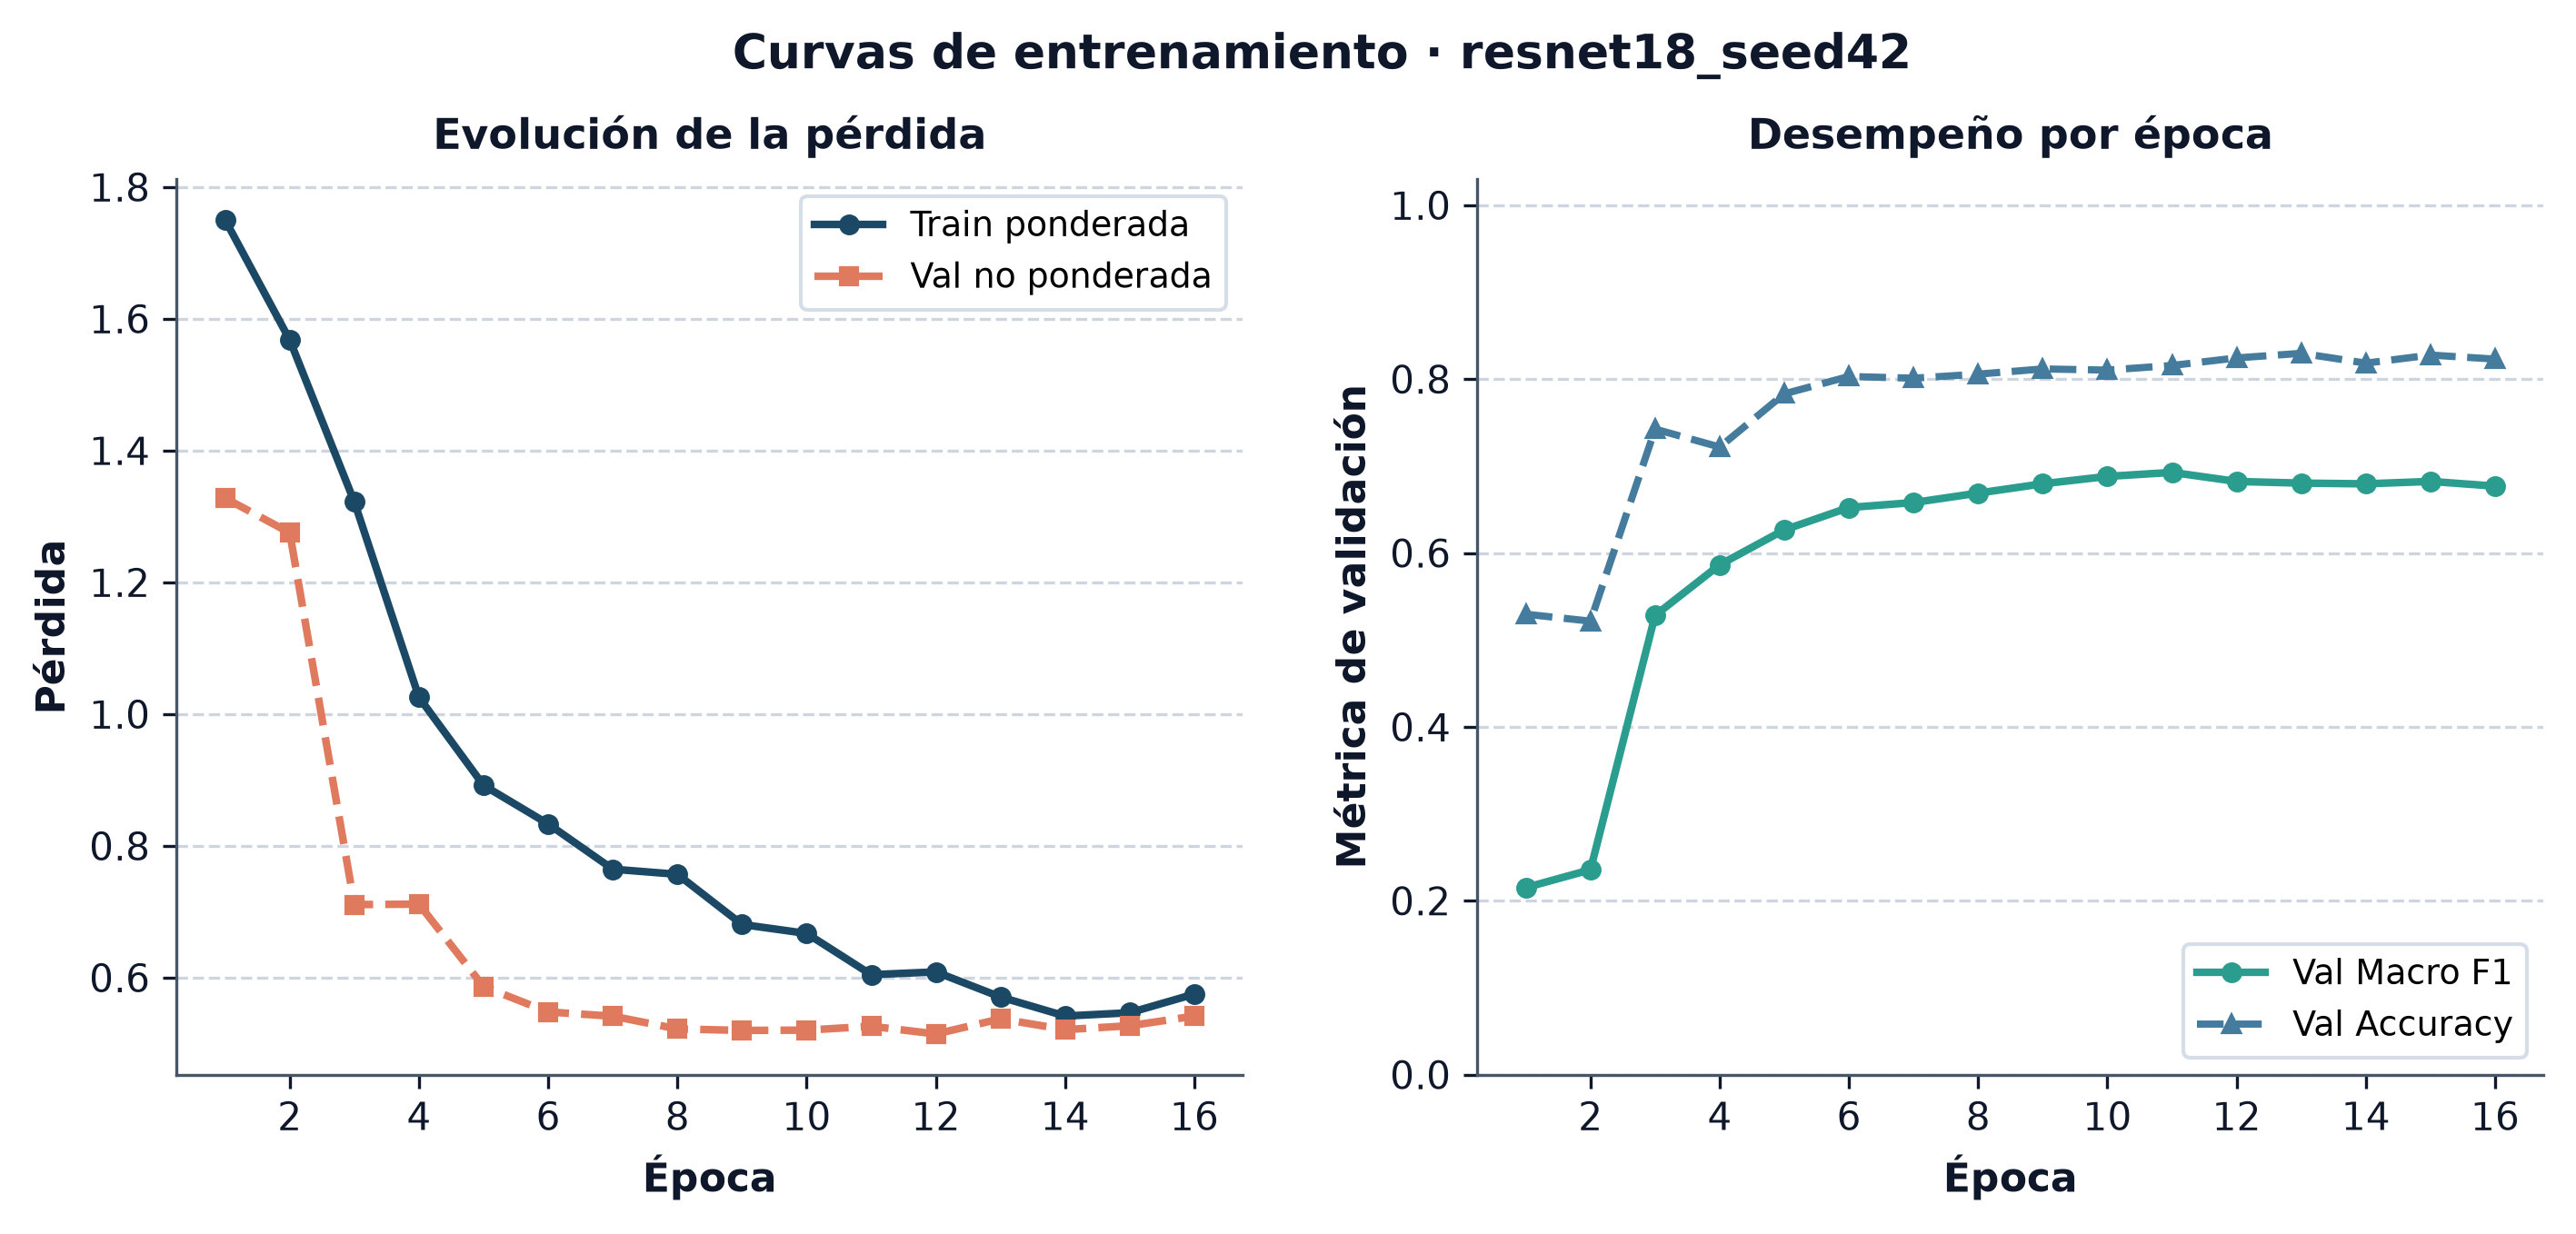
\includegraphics[width=0.92\textwidth]{curvas_resnet18_seed42.png}
\caption{Curvas reales de pérdida y métricas en validación por época para ResNet-18 (16 épocas, parada temprana; \texttt{seed=42}, \texttt{history.csv}).}
\label{fig:curvas_resnet}
\end{figure}

\begin{figure}[htbp]
\centering
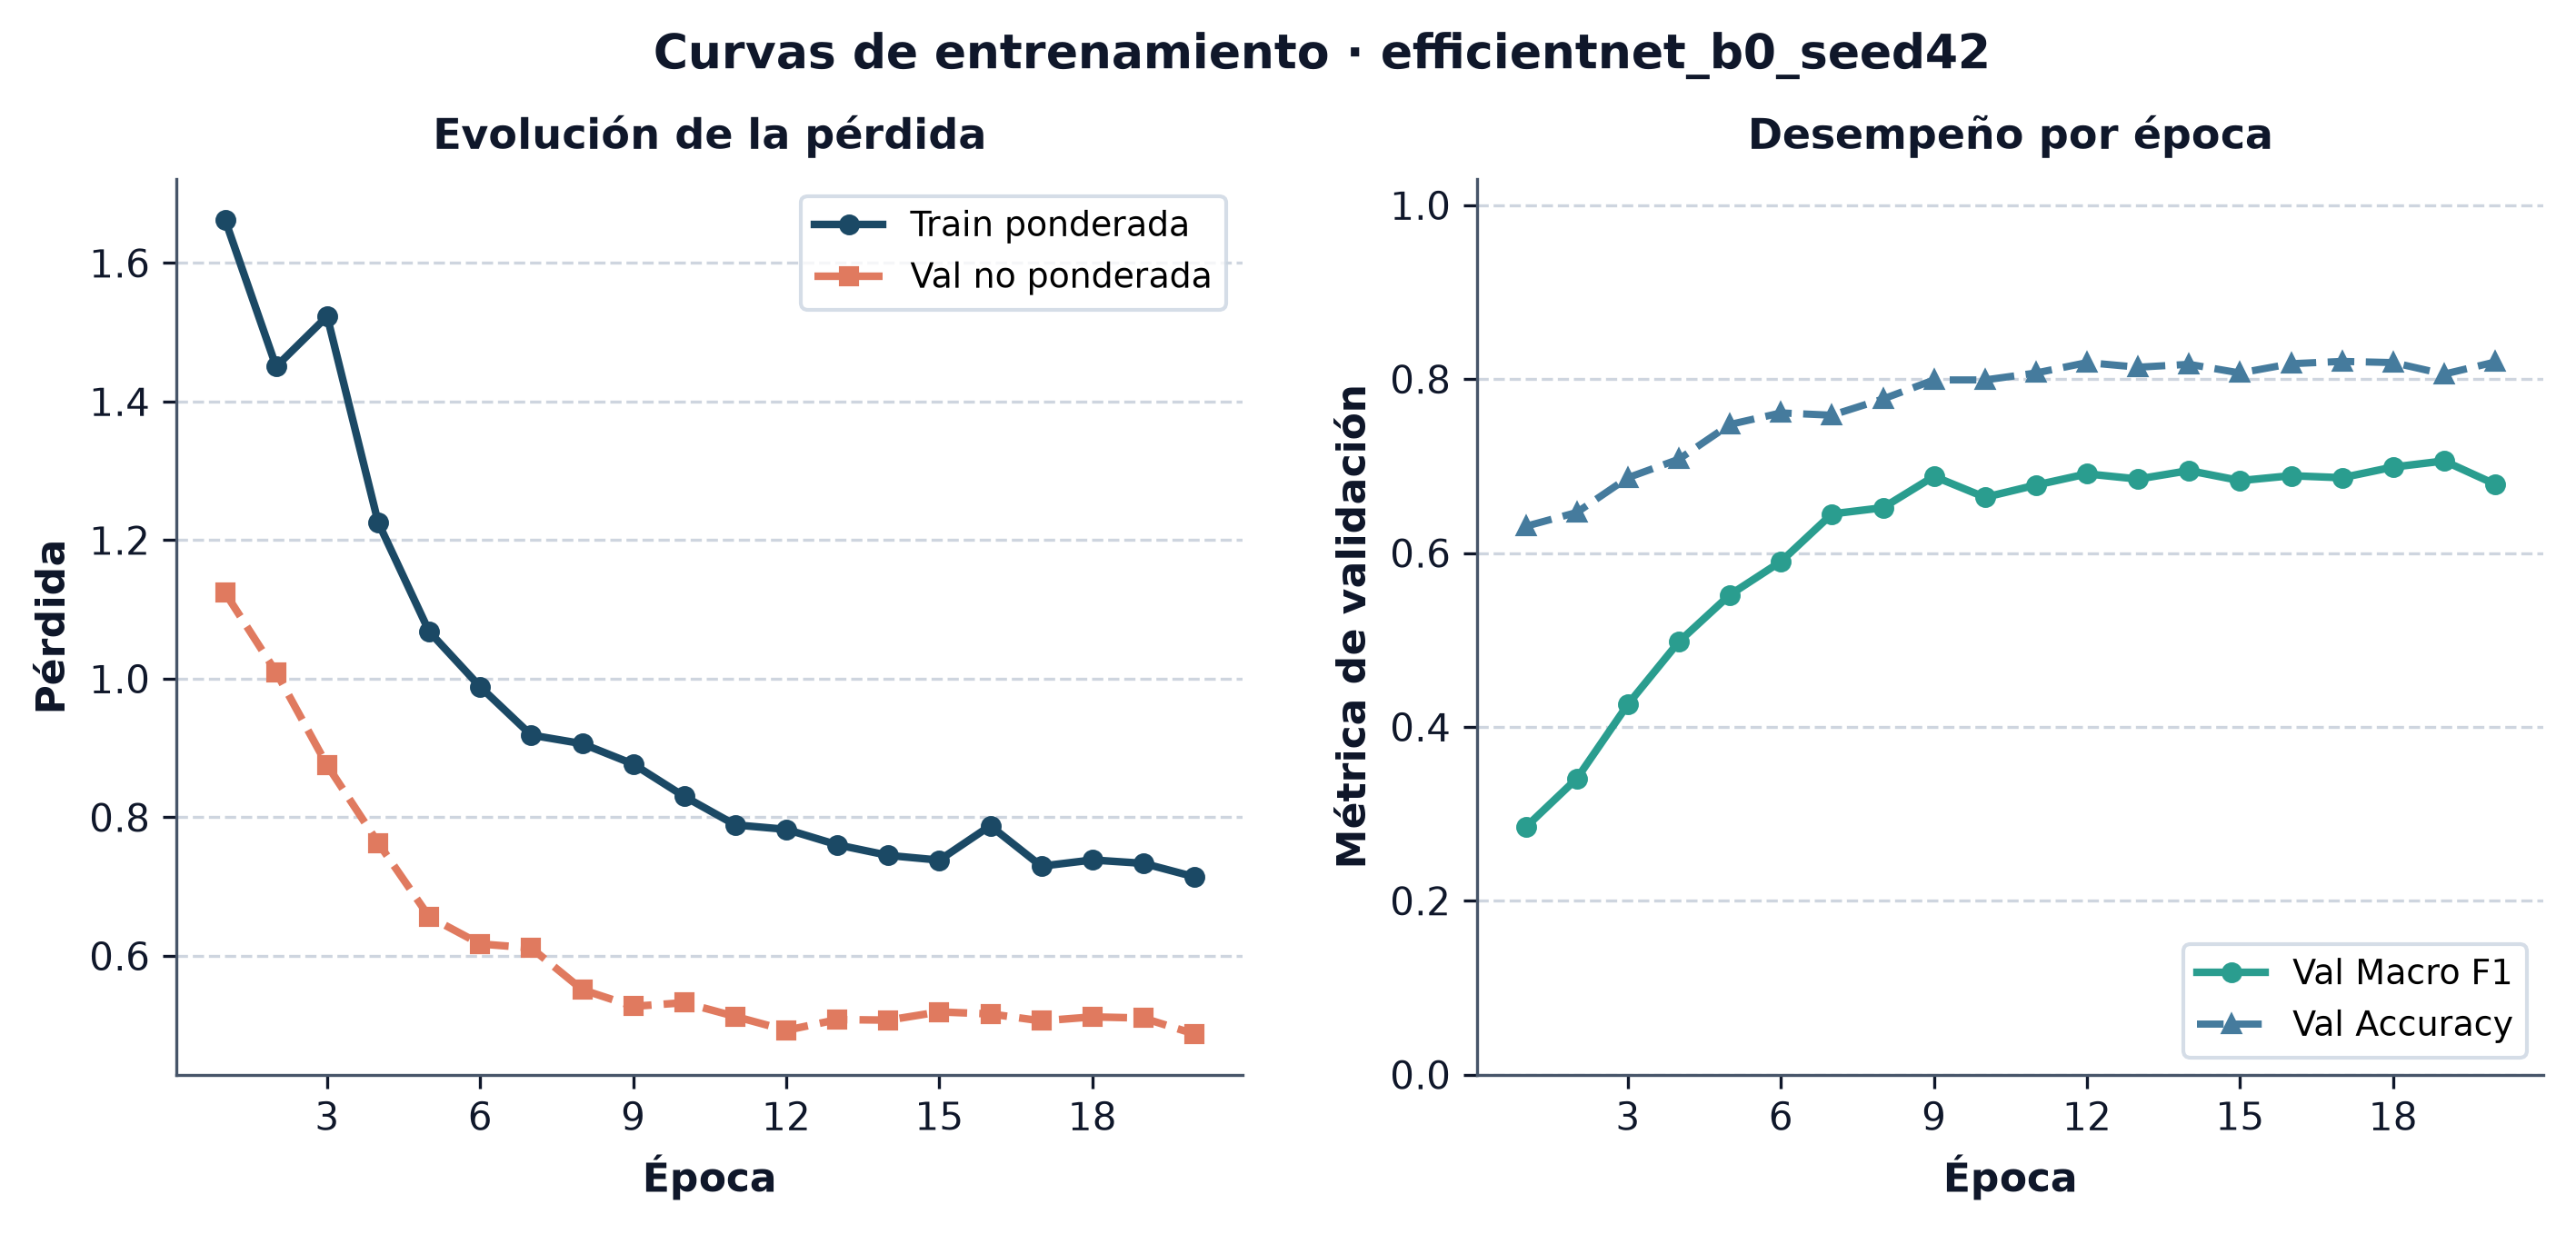
\includegraphics[width=0.92\textwidth]{curvas_efficientnet_b0_seed42.png}
\caption{Curvas reales de pérdida y métricas en validación por época para EfficientNet-B0 (20 épocas completas; \texttt{seed=42}, \texttt{history.csv}).}
\label{fig:curvas_effnet}
\end{figure}

\begin{figure}[htbp]
\centering
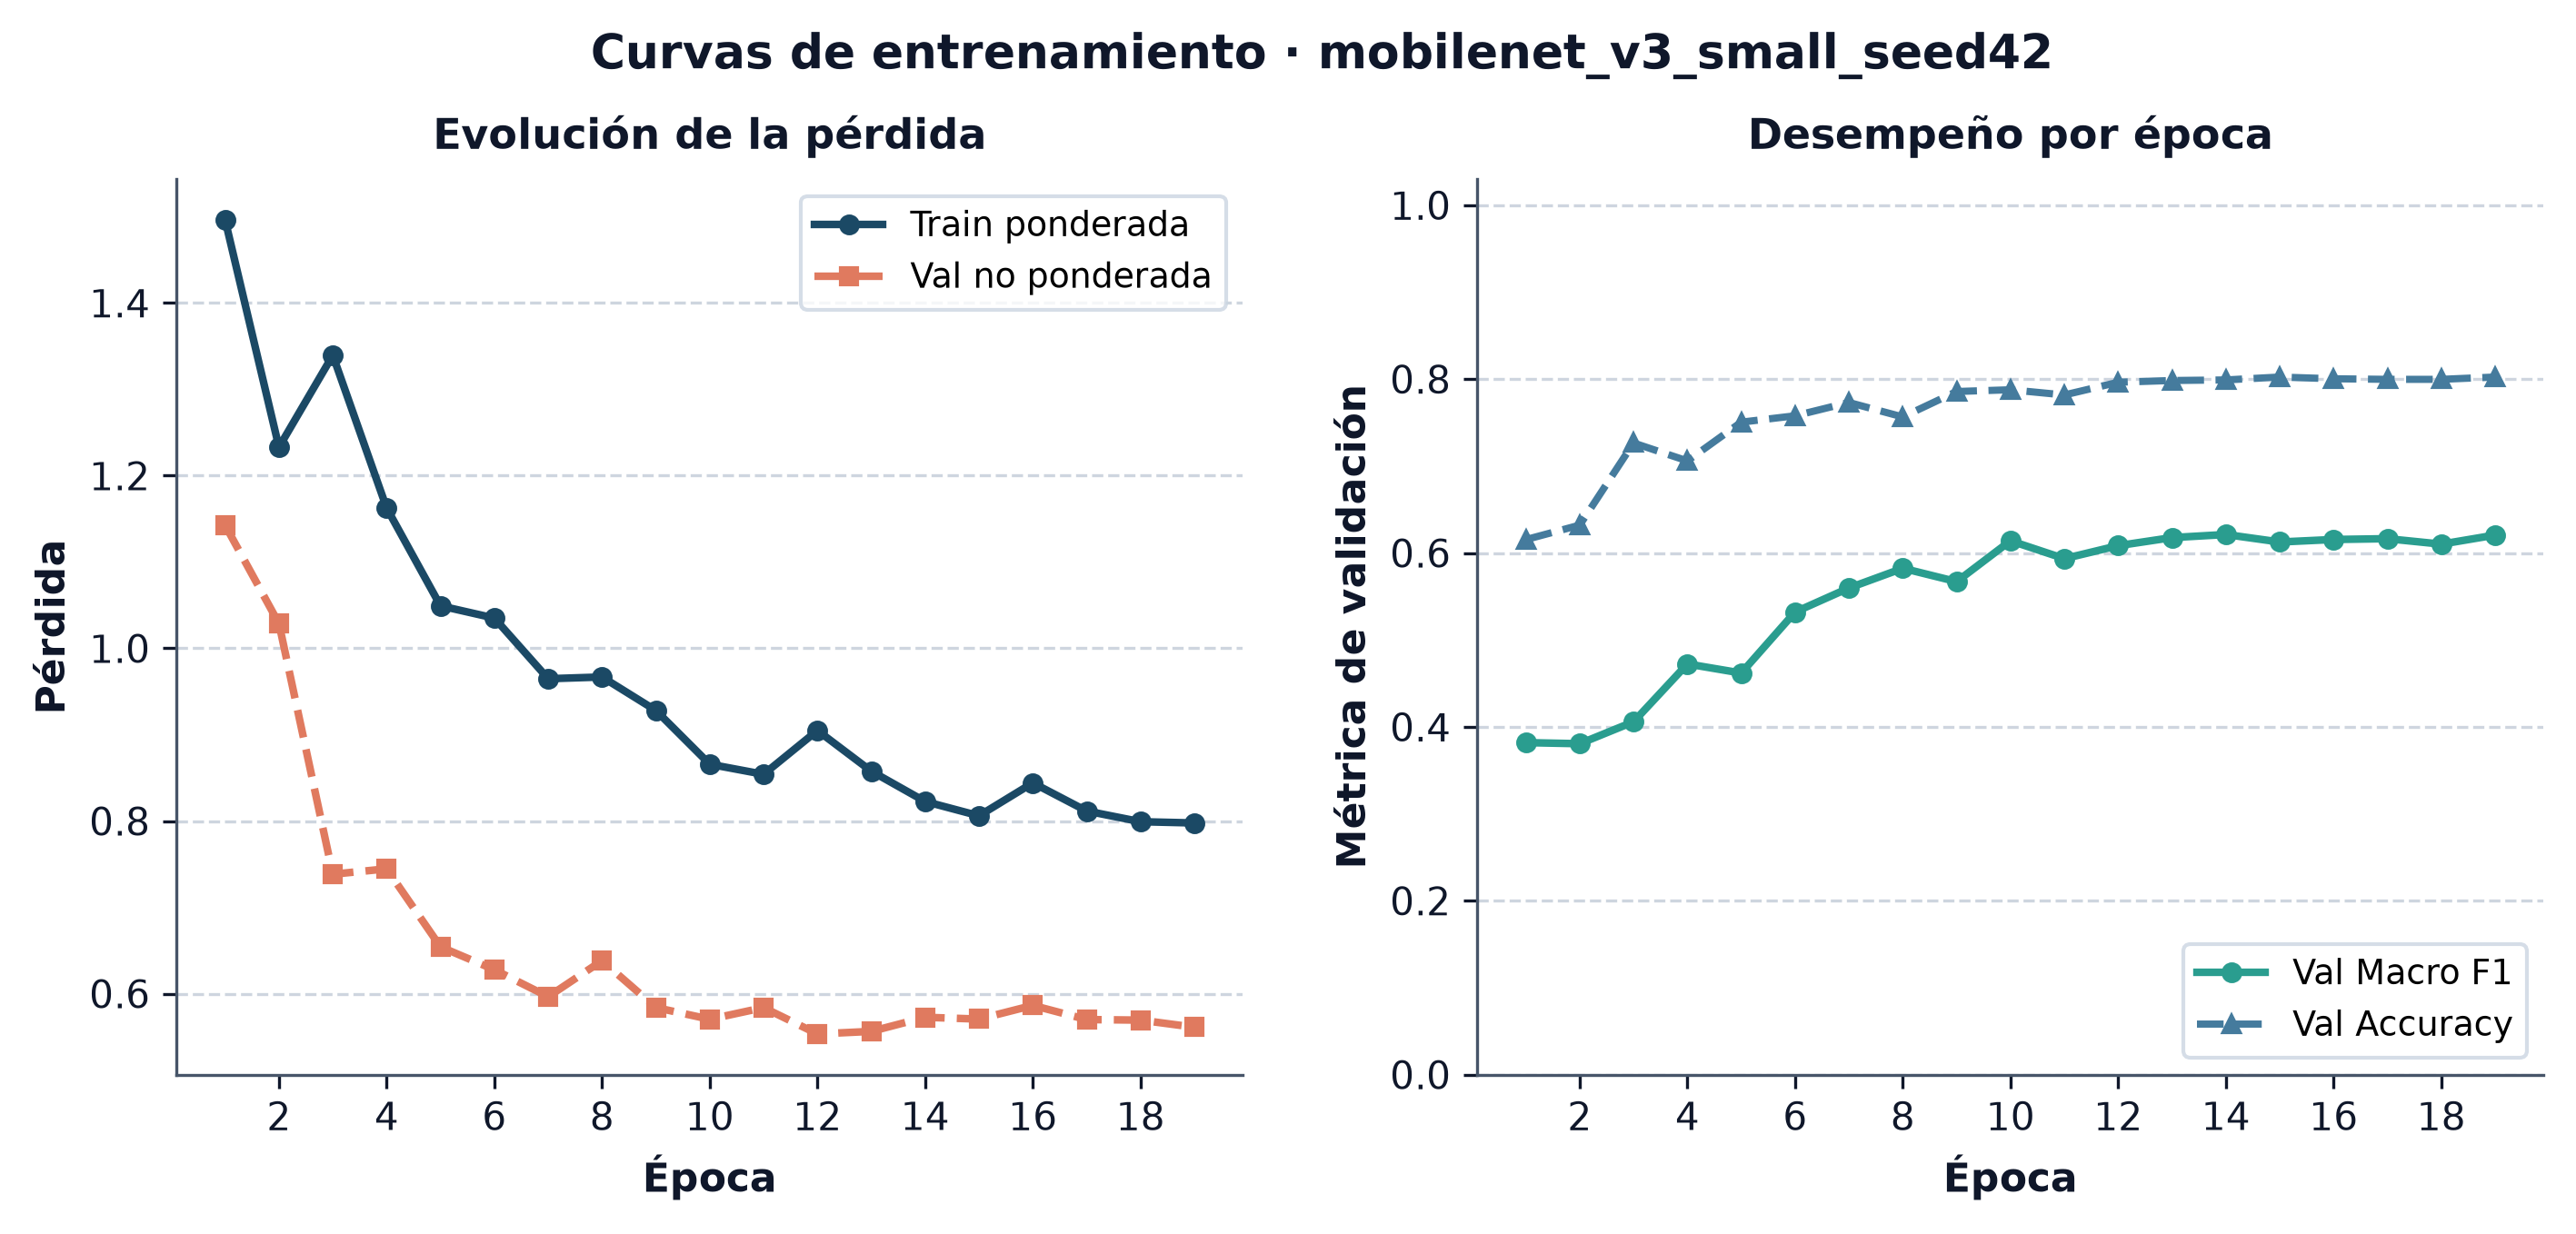
\includegraphics[width=0.92\textwidth]{curvas_mobilenet_v3_small_seed42.png}
\caption{Curvas reales de pérdida y métricas en validación por época para MobileNetV3-Small (19 épocas, parada temprana; \texttt{seed=42}, \texttt{history.csv}).}
\label{fig:curvas_mobilenet}
\end{figure}

\FloatBarrier
\subsection{Comparación global y eficiencia de los tres algoritmos}
Tras congelar los mejores checkpoints de validación (\texttt{best.pt}), se evaluó una única vez la partición \texttt{test} ($n=1\,503$) mediante \texttt{-{}-confirmar-test}. La Tabla~\ref{tab:res_global} y la Figura~\ref{fig:comp_metricas} consolidan la calidad predictiva en \texttt{test} limpio junto con el costo real medido sobre la GTX~1650.

\begin{table}[htbp]\centering\scriptsize
\setlength{\tabcolsep}{1.8pt}
\caption{Comparación global de desempeño en \texttt{test} limpio ($n=1\,503$) y eficiencia computacional entre los tres algoritmos.}
\label{tab:res_global}
\begin{tabularx}{\textwidth}{@{}>{\bfseries}l*{9}{>{\centering\arraybackslash}X}@{}}
\toprule
\textbf{Arquitectura} & \makecell{\textbf{Acc.}} & \makecell{\textbf{Macro}\\\textbf{Prec.}} & \makecell{\textbf{Macro}\\\textbf{F1}} & \makecell{\textbf{Bal.}\\\textbf{Acc.}} & \makecell{\textbf{Rec.}\\\textbf{\texttt{mel}}} & \makecell{\textbf{AUC}\\\textbf{OVR}} & \makecell{\textbf{s /}\\\textbf{época}} & \makecell{\textbf{Lat. med.}\\\textbf{(P95, ms)}} & \makecell{\textbf{VRAM}\\\textbf{(MiB)}} \\ \midrule
ResNet-18 & \textbf{0.8031} & 0.6591 & \textbf{0.6786} & \textbf{0.7174} & 0.6012 & \textbf{0.9596} & \textbf{127.5} & \makecell{\textbf{7.22}\\{\tiny (8.09)}} & 434.2 \\
EfficientNet-B0 & 0.8004 & \textbf{0.6741} & 0.6778 & 0.7025 & \textbf{0.6607} & 0.9587 & 188.6 & \makecell{24.60\\{\tiny (25.97)}} & 805.7 \\
MobileNetV3-Small & 0.7625 & 0.6474 & 0.5700 & 0.5604 & 0.4167 & 0.9407 & 156.3 & \makecell{22.40\\{\tiny (23.97)}} & \textbf{211.8} \\
\bottomrule
\end{tabularx}
\par\smallskip{\scriptsize\raggedright Nota: la latencia corresponde exclusivamente a \texttt{forward()} en GPU con \texttt{batch=1} (sin E/S ni preprocesamiento). Entre las corridas repetidas del mismo modelo en la GTX~1650 se observó dispersión operativa de $6.86$--$9.46$~ms (ResNet-18), $22.49$--$34.82$~ms (EfficientNet-B0) y $15.26$--$22.40$~ms (MobileNetV3-Small).\par}
\end{table}

\begin{figure}[htbp]
\centering
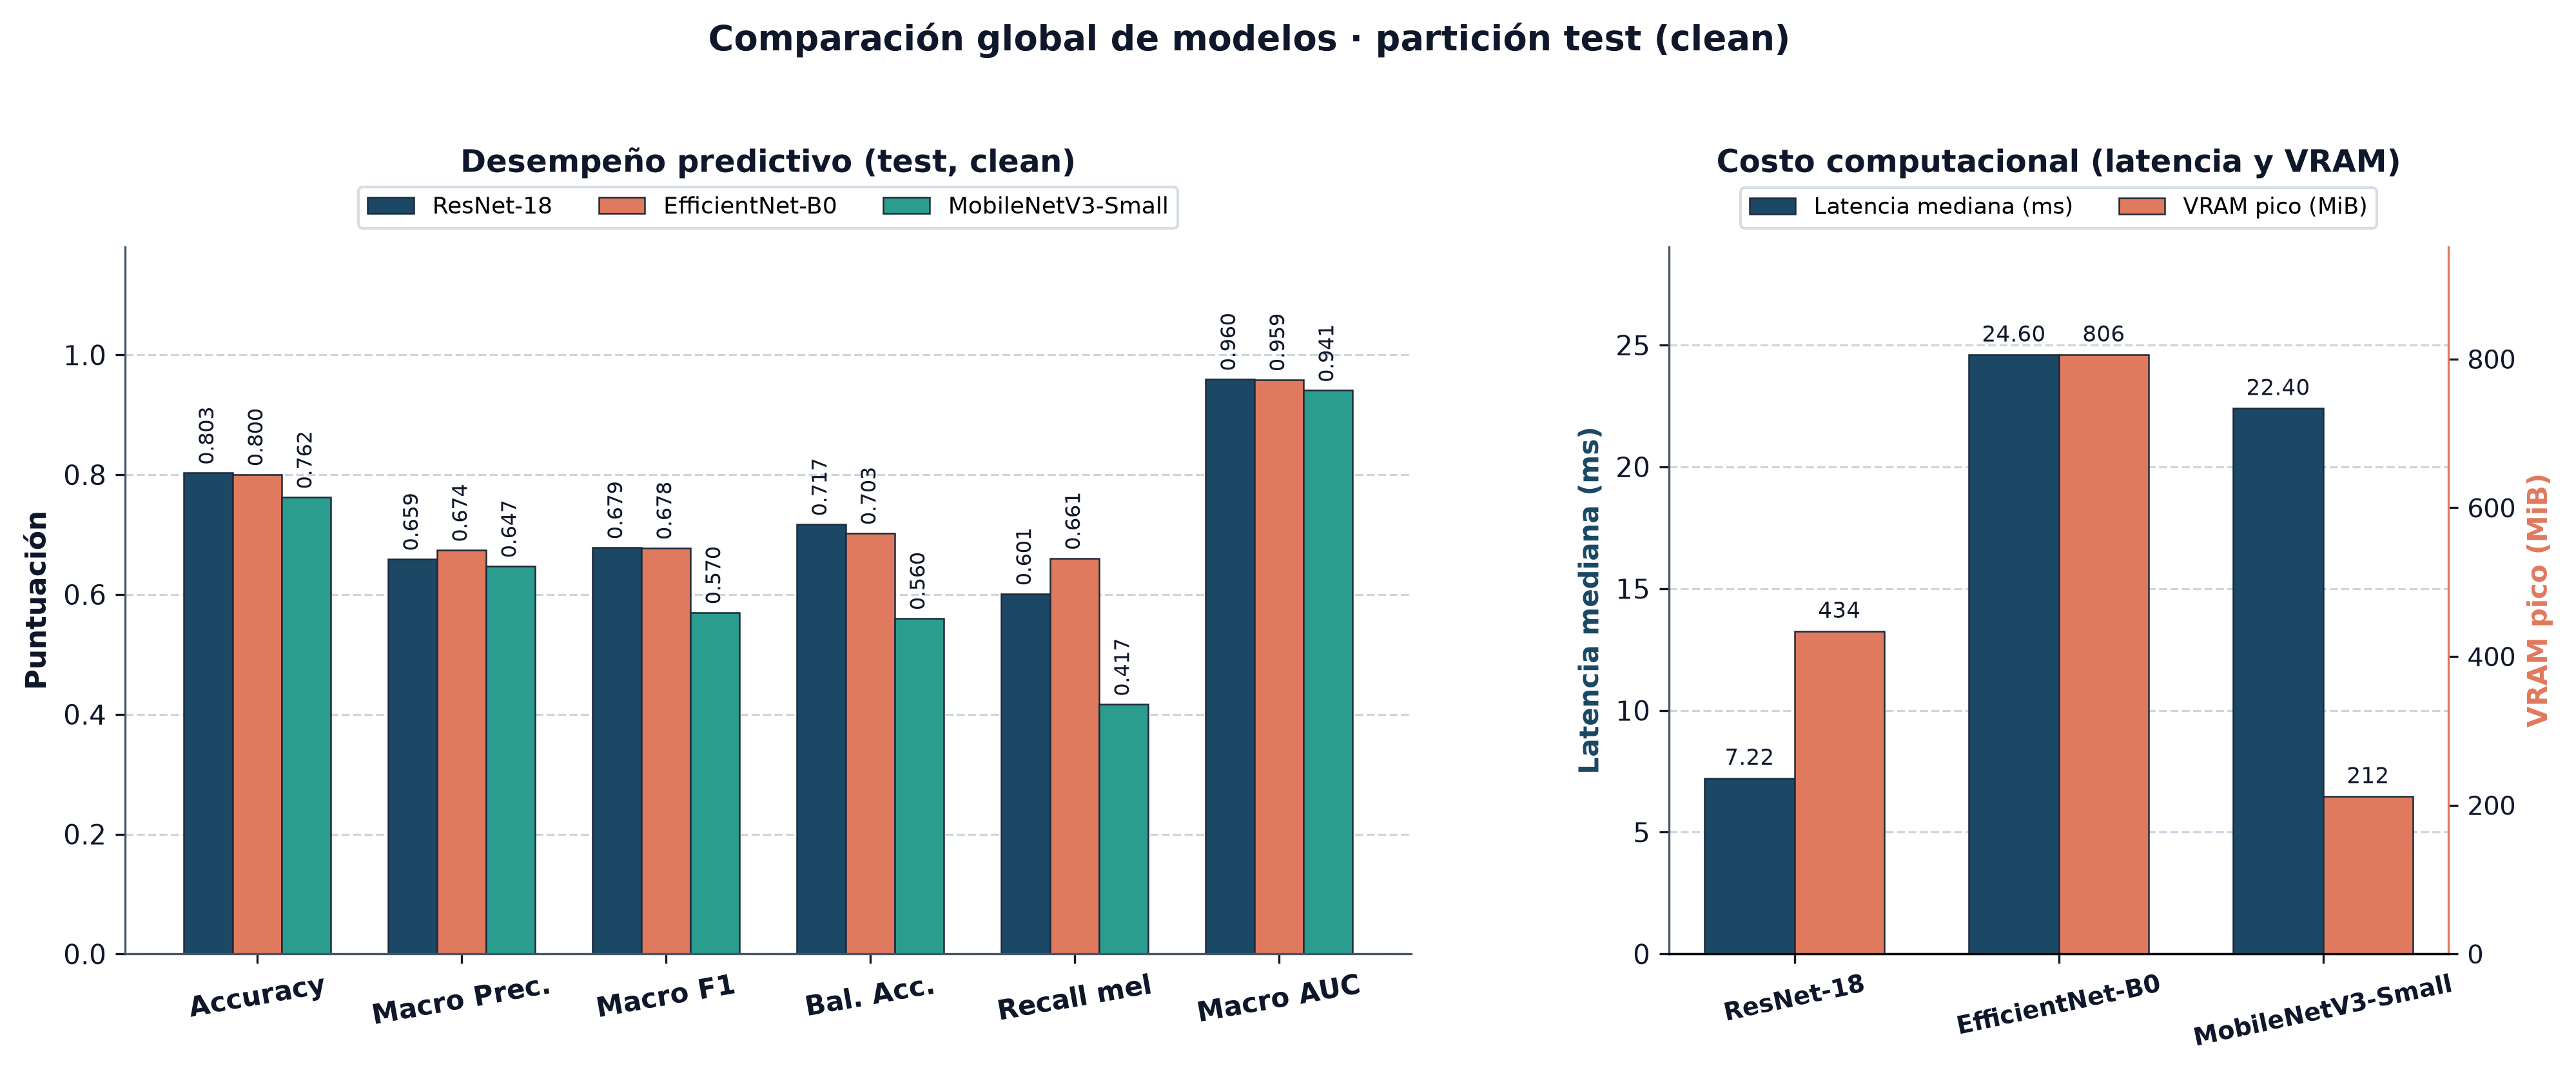
\includegraphics[width=0.96\textwidth]{comparacion_metricas.png}
\caption{Comparación visual del desempeño predictivo en \texttt{test} limpio (izquierda) y del costo computacional en GTX~1650 (derecha).}
\label{fig:comp_metricas}
\end{figure}

Los resultados globales muestran dos hallazgos relevantes. En primer lugar, bajo este protocolo común y hardware, \textbf{ResNet-18} ofrece el mejor compromiso observado desempeño--latencia (Macro~F1 = 0.6786, Macro~Prec.\ = 0.6591, \textit{Balanced Accuracy} = 0.7174, $\mathrm{AUC}_{\mathrm{OVR}}$ = 0.9596, \texttt{forward()} = 7.22~ms), frente a \textbf{EfficientNet-B0} (Macro~F1 = 0.6778, Macro~Prec.\ = 0.6741, mayor sensibilidad limpia en melanoma con 0.6607 vs.\ 0.6012). Sin embargo, la diferencia puntual de $0.00084$ en Macro~F1 entre ambas arquitecturas \textbf{no demuestra superioridad estadística ni equivalencia}: un análisis complementario por \textit{bootstrap} pareado sobre los $1\,118$ grupos independientes (\texttt{group\_id}) de \texttt{test} arroja un intervalo de confianza al 95\% de $[-0.0429, +0.0464]$. En cambio, \textbf{MobileNetV3-Small} pierde más de 10.8 puntos porcentuales en Macro~F1 (0.5700) y 15.7 puntos en \textit{Balanced Accuracy} (0.5604), aunque su \textit{Accuracy} aparente (0.7625) luzca elevada por el peso de la clase mayoritaria \texttt{nv}.

En segundo lugar, en eficiencia real sobre GPU GTX~1650 en FP32, \textbf{ResNet-18} entrena en 127.5~s/época y registra una latencia mediana de \texttt{forward()} (\texttt{batch=1}, excluyendo lectura en disco y preprocesamiento) de \textbf{7.22~ms} (P95 = 8.09~ms; rango entre corridas repetidas: $6.86$--$9.46$~ms), frente a $22.40$~ms en MobileNetV3-Small (rango $15.26$--$22.40$~ms) y $24.60$~ms en EfficientNet-B0 (rango $22.49$--$34.82$~ms). Aunque MobileNetV3-Small minimiza el pico de VRAM (211.8~MiB frente a 434.2~MiB en ResNet-18 y 805.7~MiB en EfficientNet-B0), una hipótesis interpretativa plausible (no verificada mediante perfilado de núcleos ni estudios de ablación) es que la secuencia profunda de capas separables, bloques SE y activaciones \textit{h-swish} genere mayor sobrecarga de lanzamiento de núcleos y fragmentación de accesos en CUDA que las convoluciones residuales estándar $3\times 3$ de ResNet-18 en \texttt{batch=1}.

\FloatBarrier
\subsection{Comparación detallada por categoría diagnóstica}
Debido al desbalance de $58.3:1$, la Tabla~\ref{tab:res_clases} desglosa \textit{Precision}, \textit{Recall}, F1 y $\mathrm{AUC}_{\mathrm{OVR}}$ sobre las siete categorías diagnósticas de \texttt{test} ($n=1\,503$), complementada con las matrices de confusión (Figuras~\ref{fig:conf_resnet}--\ref{fig:conf_mobilenet}) y las curvas ROC OVR comparativas e individuales (Figuras~\ref{fig:roc_comp} y~\ref{fig:roc_resnet}--\ref{fig:roc_mobilenet}).

\begin{table}[htbp]\centering\scriptsize
\setlength{\tabcolsep}{1.3pt}
\caption{Desglose comparativo de Precision (P), Recall (R), F1 y AUC OVR por clase en el conjunto fijo \texttt{test} ($n=1\,503$).}
\label{tab:res_clases}
\begin{tabular*}{\textwidth}{@{\extracolsep{\fill}}>{\ttfamily}lrr*{12}{r}@{}}
\toprule
\textrm{\textbf{Clase}} & \makecell[r]{\textbf{Sop.}\\\textbf{\texttt{test}}} & \makecell[r]{\textbf{$w_c$}\\\textbf{\texttt{train}}} & \multicolumn{4}{c}{\textbf{ResNet-18}} & \multicolumn{4}{c}{\textbf{EfficientNet-B0}} & \multicolumn{4}{c}{\textbf{MobileNetV3-Small}} \\
\cmidrule(lr){4-7}\cmidrule(lr){8-11}\cmidrule(lr){12-15}
 & & & \textbf{P} & \textbf{R} & \textbf{F1} & \textbf{AUC} & \textbf{P} & \textbf{R} & \textbf{F1} & \textbf{AUC} & \textbf{P} & \textbf{R} & \textbf{F1} & \textbf{AUC} \\ \midrule
akiec & 49 & 4.3916 & 0.6889 & \textbf{0.6327} & 0.6596 & 0.9791 & \textbf{0.8571} & 0.6122 & \textbf{0.7143} & \textbf{0.9878} & 0.7273 & 0.1633 & 0.2667 & 0.9743 \\
bcc & 78 & 2.7891 & \textbf{0.7812} & 0.6410 & \textbf{0.7042} & \textbf{0.9798} & 0.7500 & 0.6154 & 0.6761 & 0.9743 & 0.6118 & \textbf{0.6667} & 0.6380 & 0.9720 \\
bkl & 165 & 1.3021 & 0.5967 & 0.6545 & 0.6243 & \textbf{0.9320} & \textbf{0.6054} & \textbf{0.6788} & \textbf{0.6400} & 0.9261 & 0.4589 & 0.6424 & 0.5354 & 0.8881 \\
df & 17 & 12.5161 & 0.4000 & \textbf{0.7059} & \textbf{0.5106} & \textbf{0.9882} & 0.3750 & 0.5294 & 0.4390 & 0.9708 & \textbf{0.5556} & 0.2941 & 0.3846 & 0.9692 \\
mel & 168 & 1.2853 & \textbf{0.5233} & 0.6012 & 0.5596 & 0.8947 & 0.4868 & \textbf{0.6607} & \textbf{0.5606} & \textbf{0.9113} & 0.4698 & 0.4167 & 0.4416 & 0.8594 \\
nv & 1\,005 & 0.2133 & 0.9200 & 0.8816 & \textbf{0.9004} & 0.9458 & \textbf{0.9297} & 0.8687 & 0.8981 & \textbf{0.9488} & 0.8906 & \textbf{0.8826} & 0.8866 & 0.9281 \\
vasc & 21 & 10.0129 & 0.7037 & 0.9048 & 0.7917 & \textbf{0.9976} & 0.7143 & \textbf{0.9524} & 0.8163 & 0.9921 & \textbf{0.8182} & 0.8571 & \textbf{0.8372} & 0.9938 \\ \midrule
\textrm{\textbf{Macro}} & \textbf{1\,503} & --- & 0.6591 & \textbf{0.7174} & \textbf{0.6786} & \textbf{0.9596} & \textbf{0.6741} & 0.7025 & 0.6778 & 0.9587 & 0.6474 & 0.5604 & 0.5700 & 0.9407 \\
\bottomrule
\end{tabular*}
\end{table}

\begin{figure}[htbp]
\centering
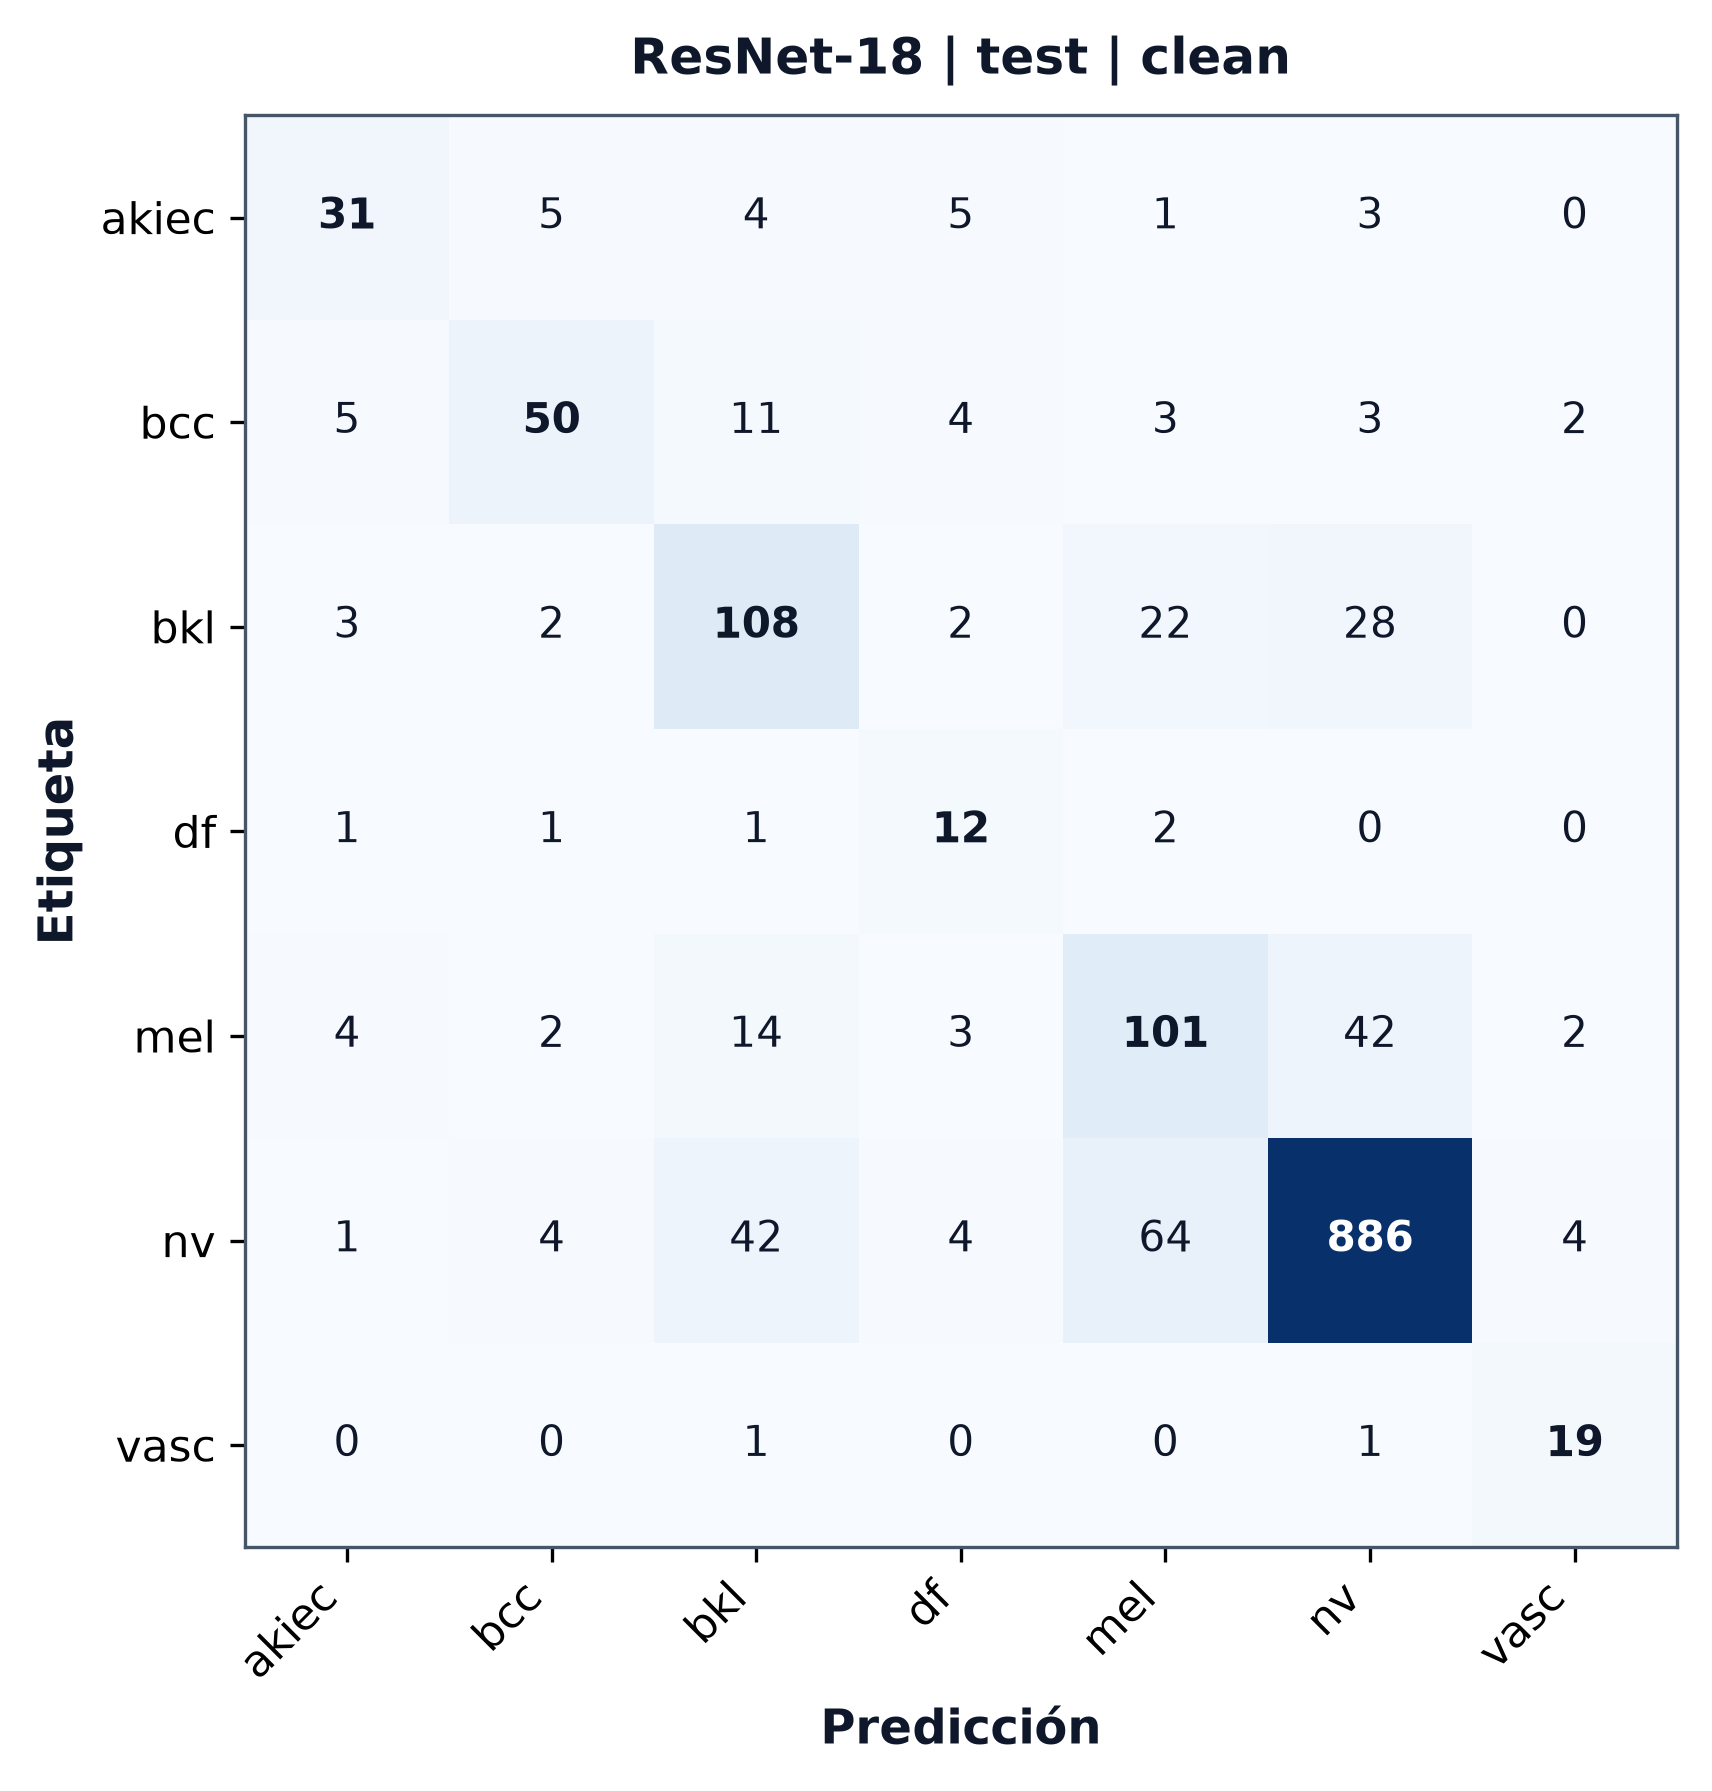
\includegraphics[width=0.68\textwidth]{confusion_resnet18_42_test_clean.png}
\caption{Matriz de confusión $7\times 7$ de ResNet-18 en \texttt{test} limpio ($n=1\,503$, \texttt{seed=42}).}
\label{fig:conf_resnet}
\end{figure}

\begin{figure}[htbp]
\centering
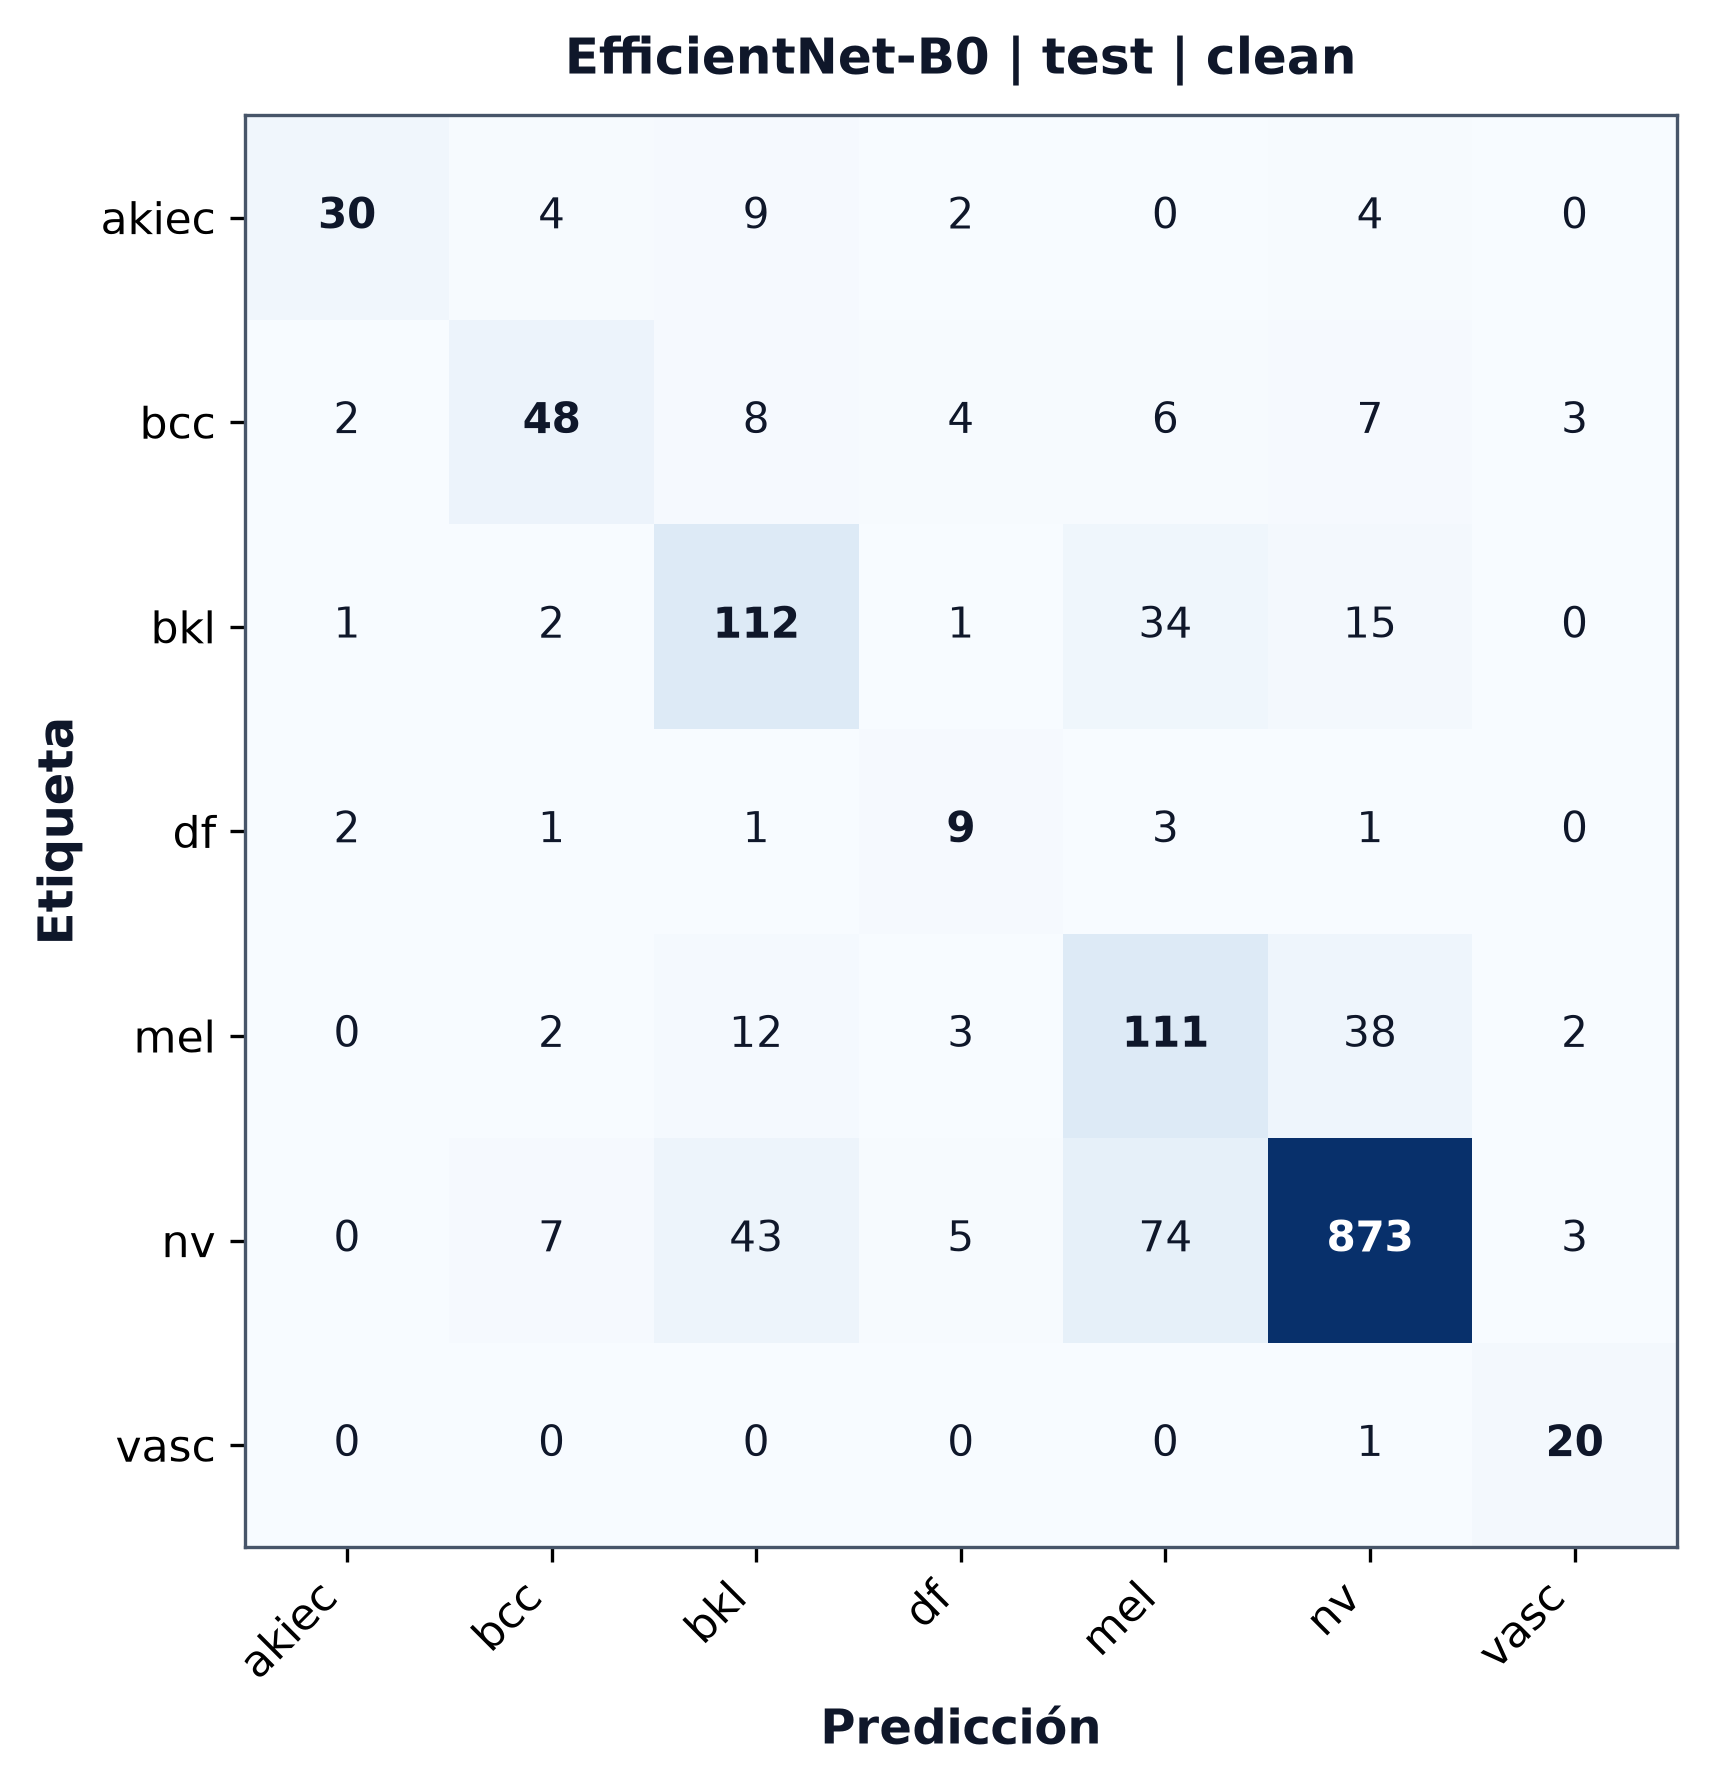
\includegraphics[width=0.68\textwidth]{confusion_efficientnet_b0_42_test_clean.png}
\caption{Matriz de confusión $7\times 7$ de EfficientNet-B0 en \texttt{test} limpio ($n=1\,503$, \texttt{seed=42}).}
\label{fig:conf_effnet}
\end{figure}

\begin{figure}[htbp]
\centering
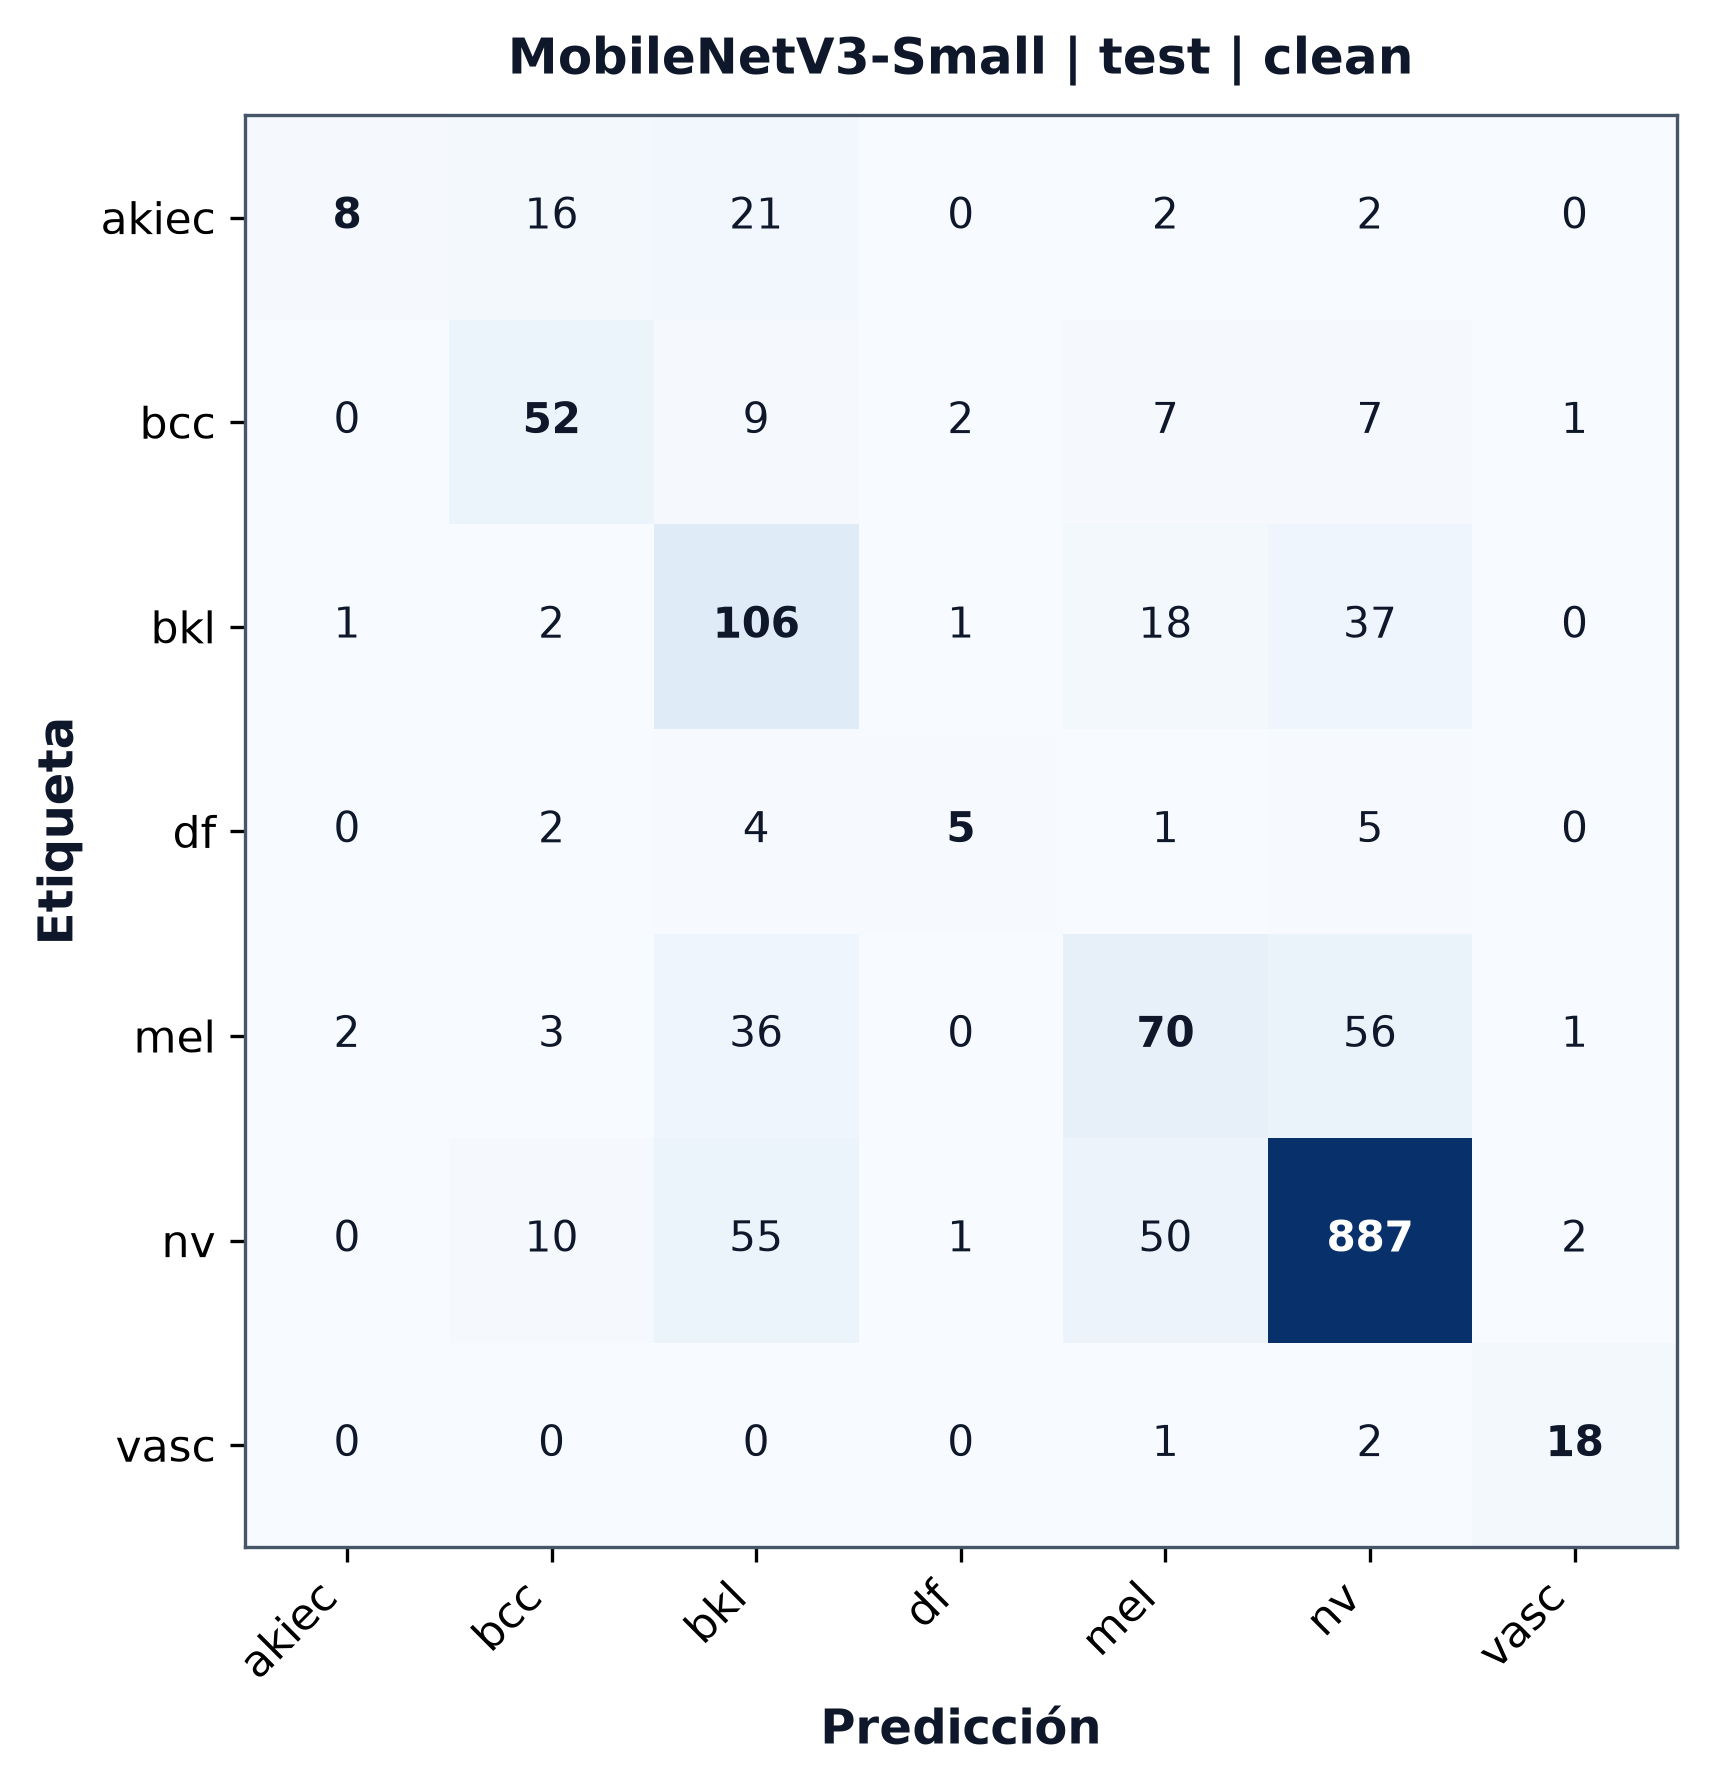
\includegraphics[width=0.68\textwidth]{confusion_mobilenet_v3_small_42_test_clean.png}
\caption{Matriz de confusión $7\times 7$ de MobileNetV3-Small en \texttt{test} limpio ($n=1\,503$, \texttt{seed=42}).}
\label{fig:conf_mobilenet}
\end{figure}
\FloatBarrier

El análisis por categoría revela dónde se origina la brecha entre modelos:
\begin{itemize}[leftmargin=1.4em,itemsep=3pt]
\item \textbf{Melanoma (\texttt{mel}, $n=168$):} es la categoría más crítica y difícil de separar. EfficientNet-B0 alcanza la mayor sensibilidad (0.6607; 111/168 aciertos) y F1 (0.5606) con \textit{Precision} de 0.4868, mientras ResNet-18 logra mayor \textit{Precision} (0.5233), \textit{Recall} de 0.6012 (101/168 aciertos; 92 falsos positivos, 67 falsos negativos) y F1 muy cercano (0.5596) gracias a menor tasa de confusión desde \texttt{nv} (64 casos frente a 74 en EfficientNet-B0) y \texttt{bkl} (22 frente a 34). MobileNetV3-Small cae a 0.4167 de sensibilidad (solo 70/168, \textit{Precision} = 0.4698), confundiendo 56 melanomas con \texttt{nv} y 36 con \texttt{bkl}.
\item \textbf{Clases minoritarias (\texttt{akiec}, \texttt{df}, \texttt{vasc}):} en \texttt{vasc} ($n=21$), las tres redes logran alta separabilidad (F1 entre 0.7917 y 0.8372; 18--20 aciertos). En cambio, en \texttt{akiec} ($n=49$) y \texttt{df} ($n=17$) MobileNetV3-Small colapsa en cobertura: aunque mantiene \textit{Precision} moderada (0.7273 en \texttt{akiec}, 0.5556 en \texttt{df}), solo acierta 8/49 en \texttt{akiec} (\textit{Recall} = 0.1633, F1 = 0.2667, derivando 21 casos a \texttt{bkl} y 16 a \texttt{bcc}) y 5/17 en \texttt{df} (\textit{Recall} = 0.2941, F1 = 0.3846). ResNet-18 lidera en \texttt{df} (F1 = 0.5106, \textit{Recall} = 0.7059; 12/17) y \texttt{bcc} (F1 = 0.7042, \textit{Precision} = 0.7812), mientras EfficientNet-B0 lidera en \texttt{akiec} (P = 0.8571, F1 = 0.7143) y \texttt{bkl} (P = 0.6054, F1 = 0.6400).
\item \textbf{Clase mayoritaria (\texttt{nv}, $n=1\,005$):} las tres arquitecturas muestran comportamiento homogéneo (\textit{Precision} entre 0.8906 y 0.9297; F1 entre 0.8866 y 0.9004), confirmando que el uso de pesos $w_c$ evita el colapso hacia \texttt{nv}, aunque persiste una confusión bidireccional moderada en la frontera pigmentada \texttt{nv}--\texttt{mel}--\texttt{bkl}.
\end{itemize}

\begin{figure}[htbp]
\centering
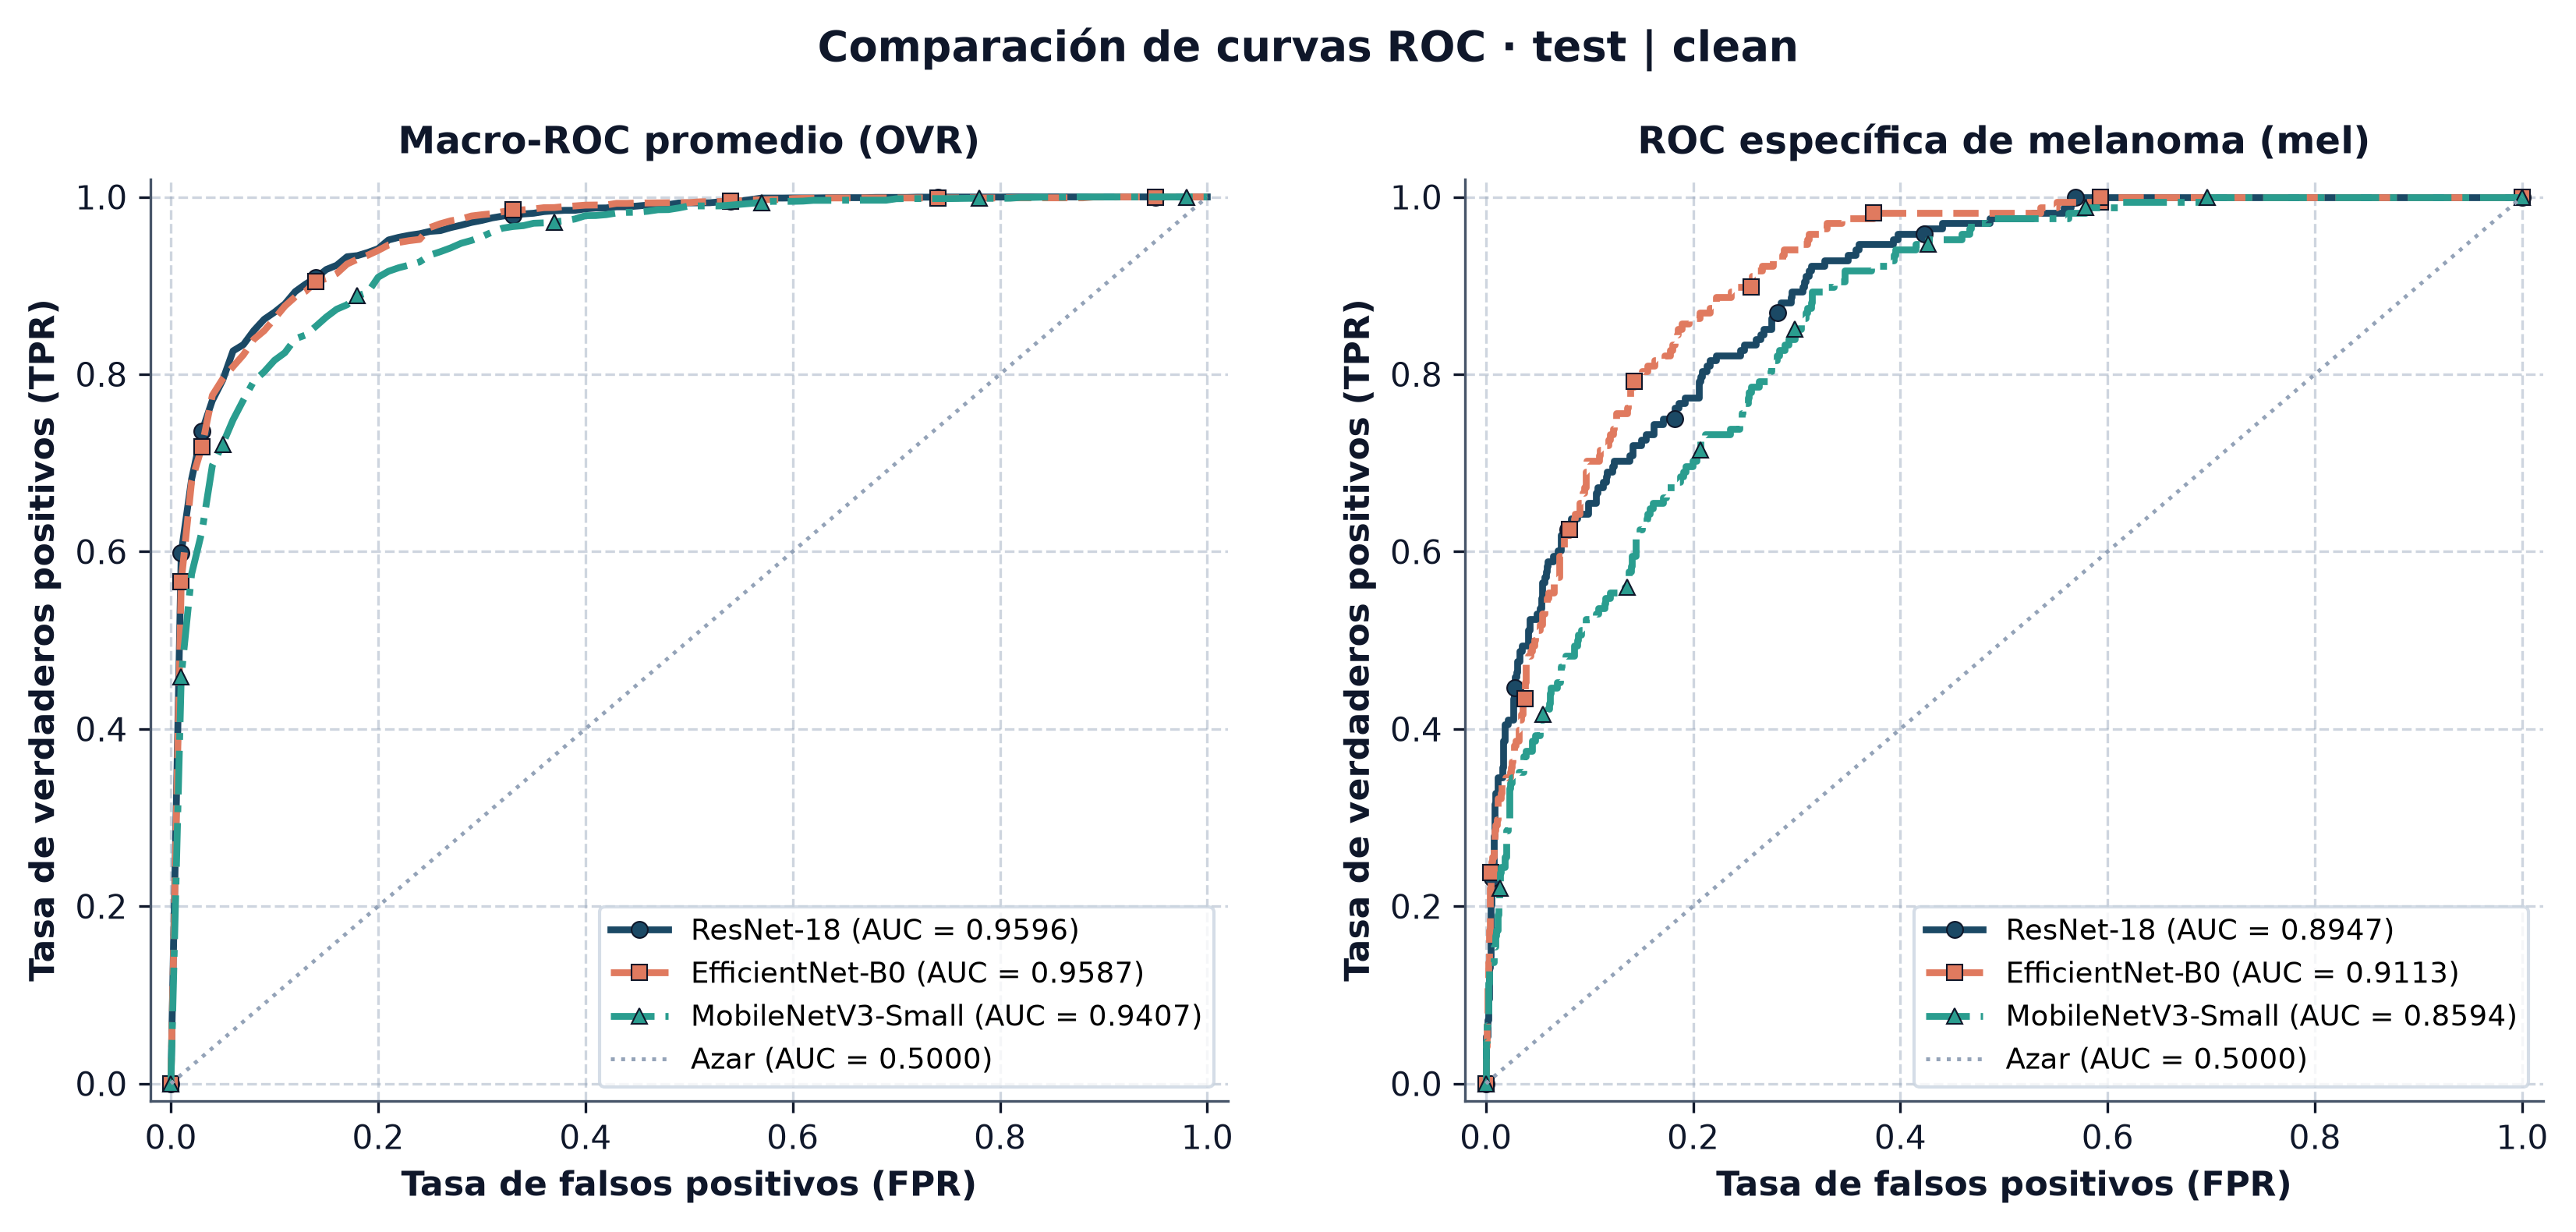
\includegraphics[width=0.96\textwidth]{roc_comparativa_test_clean.png}
\caption{Comparación de curvas ROC OVR macro-promedio (izquierda) y específica para melanoma (derecha) en \texttt{test} limpio.}
\label{fig:roc_comp}
\end{figure}

\begin{figure}[htbp]
\centering
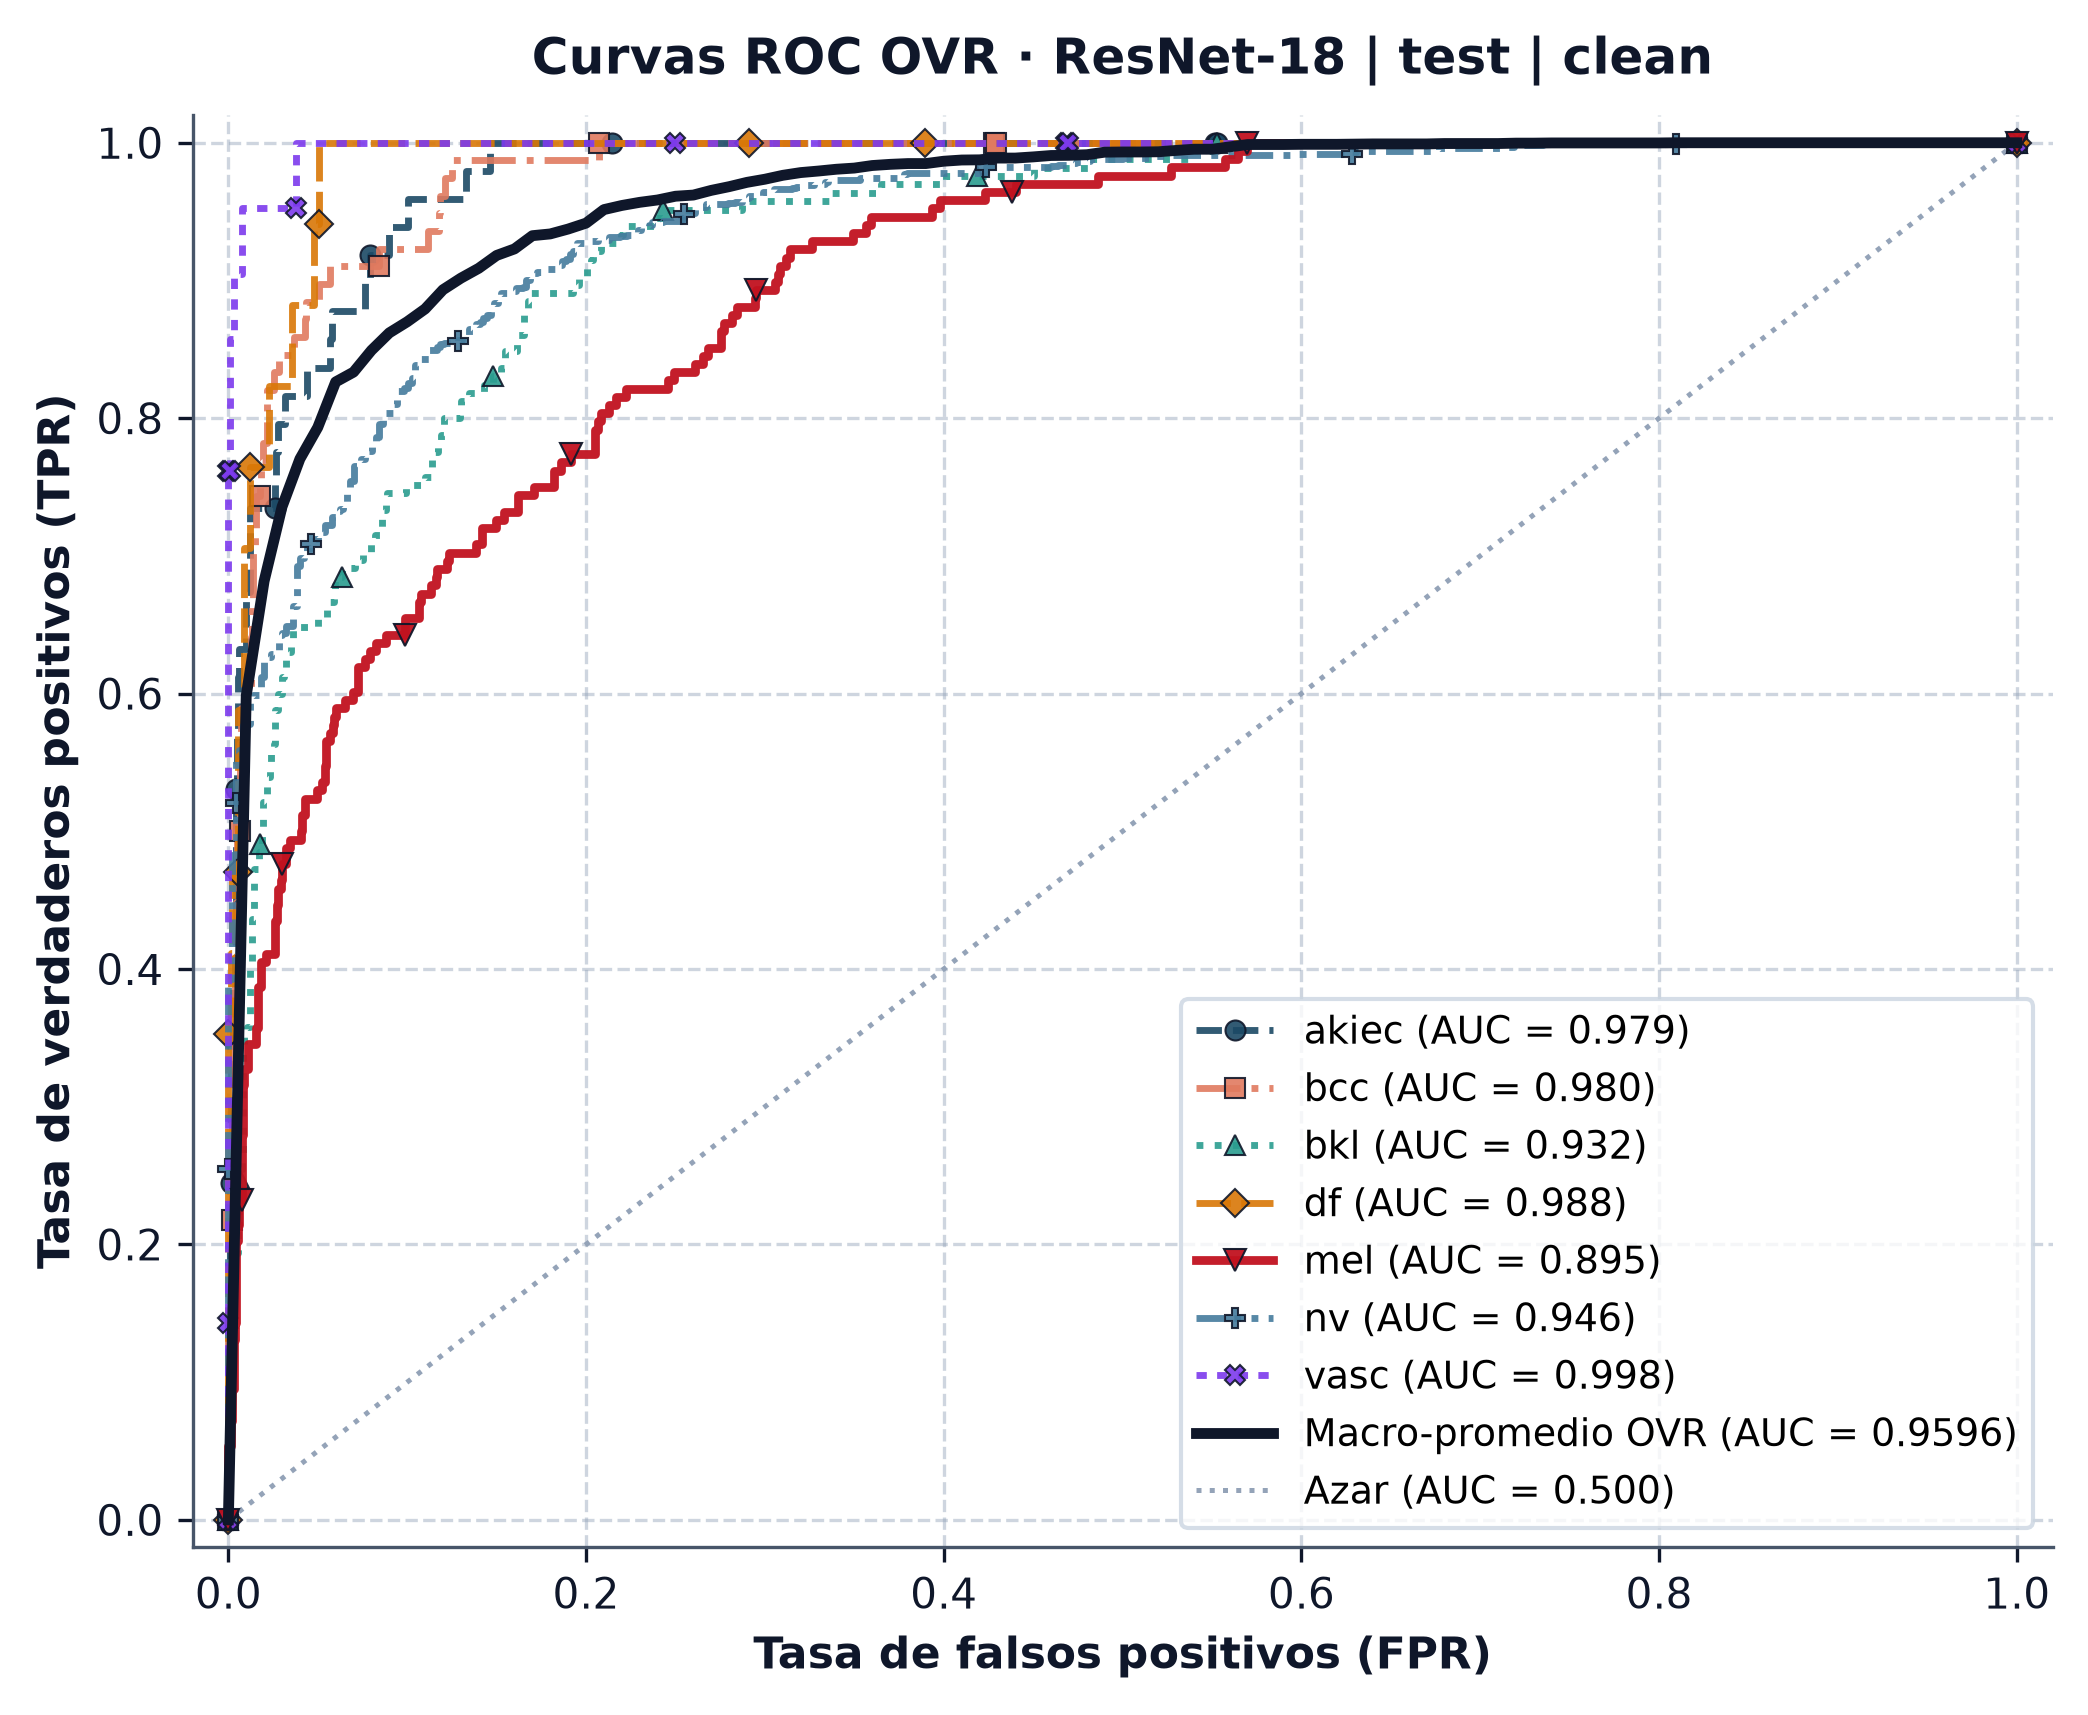
\includegraphics[width=0.78\textwidth]{roc_resnet18_42_test_clean.png}
\caption{Curvas ROC uno contra el resto (OVR) por clase en \texttt{test} limpio para ResNet-18 (\texttt{seed=42}).}
\label{fig:roc_resnet}
\end{figure}

\begin{figure}[htbp]
\centering
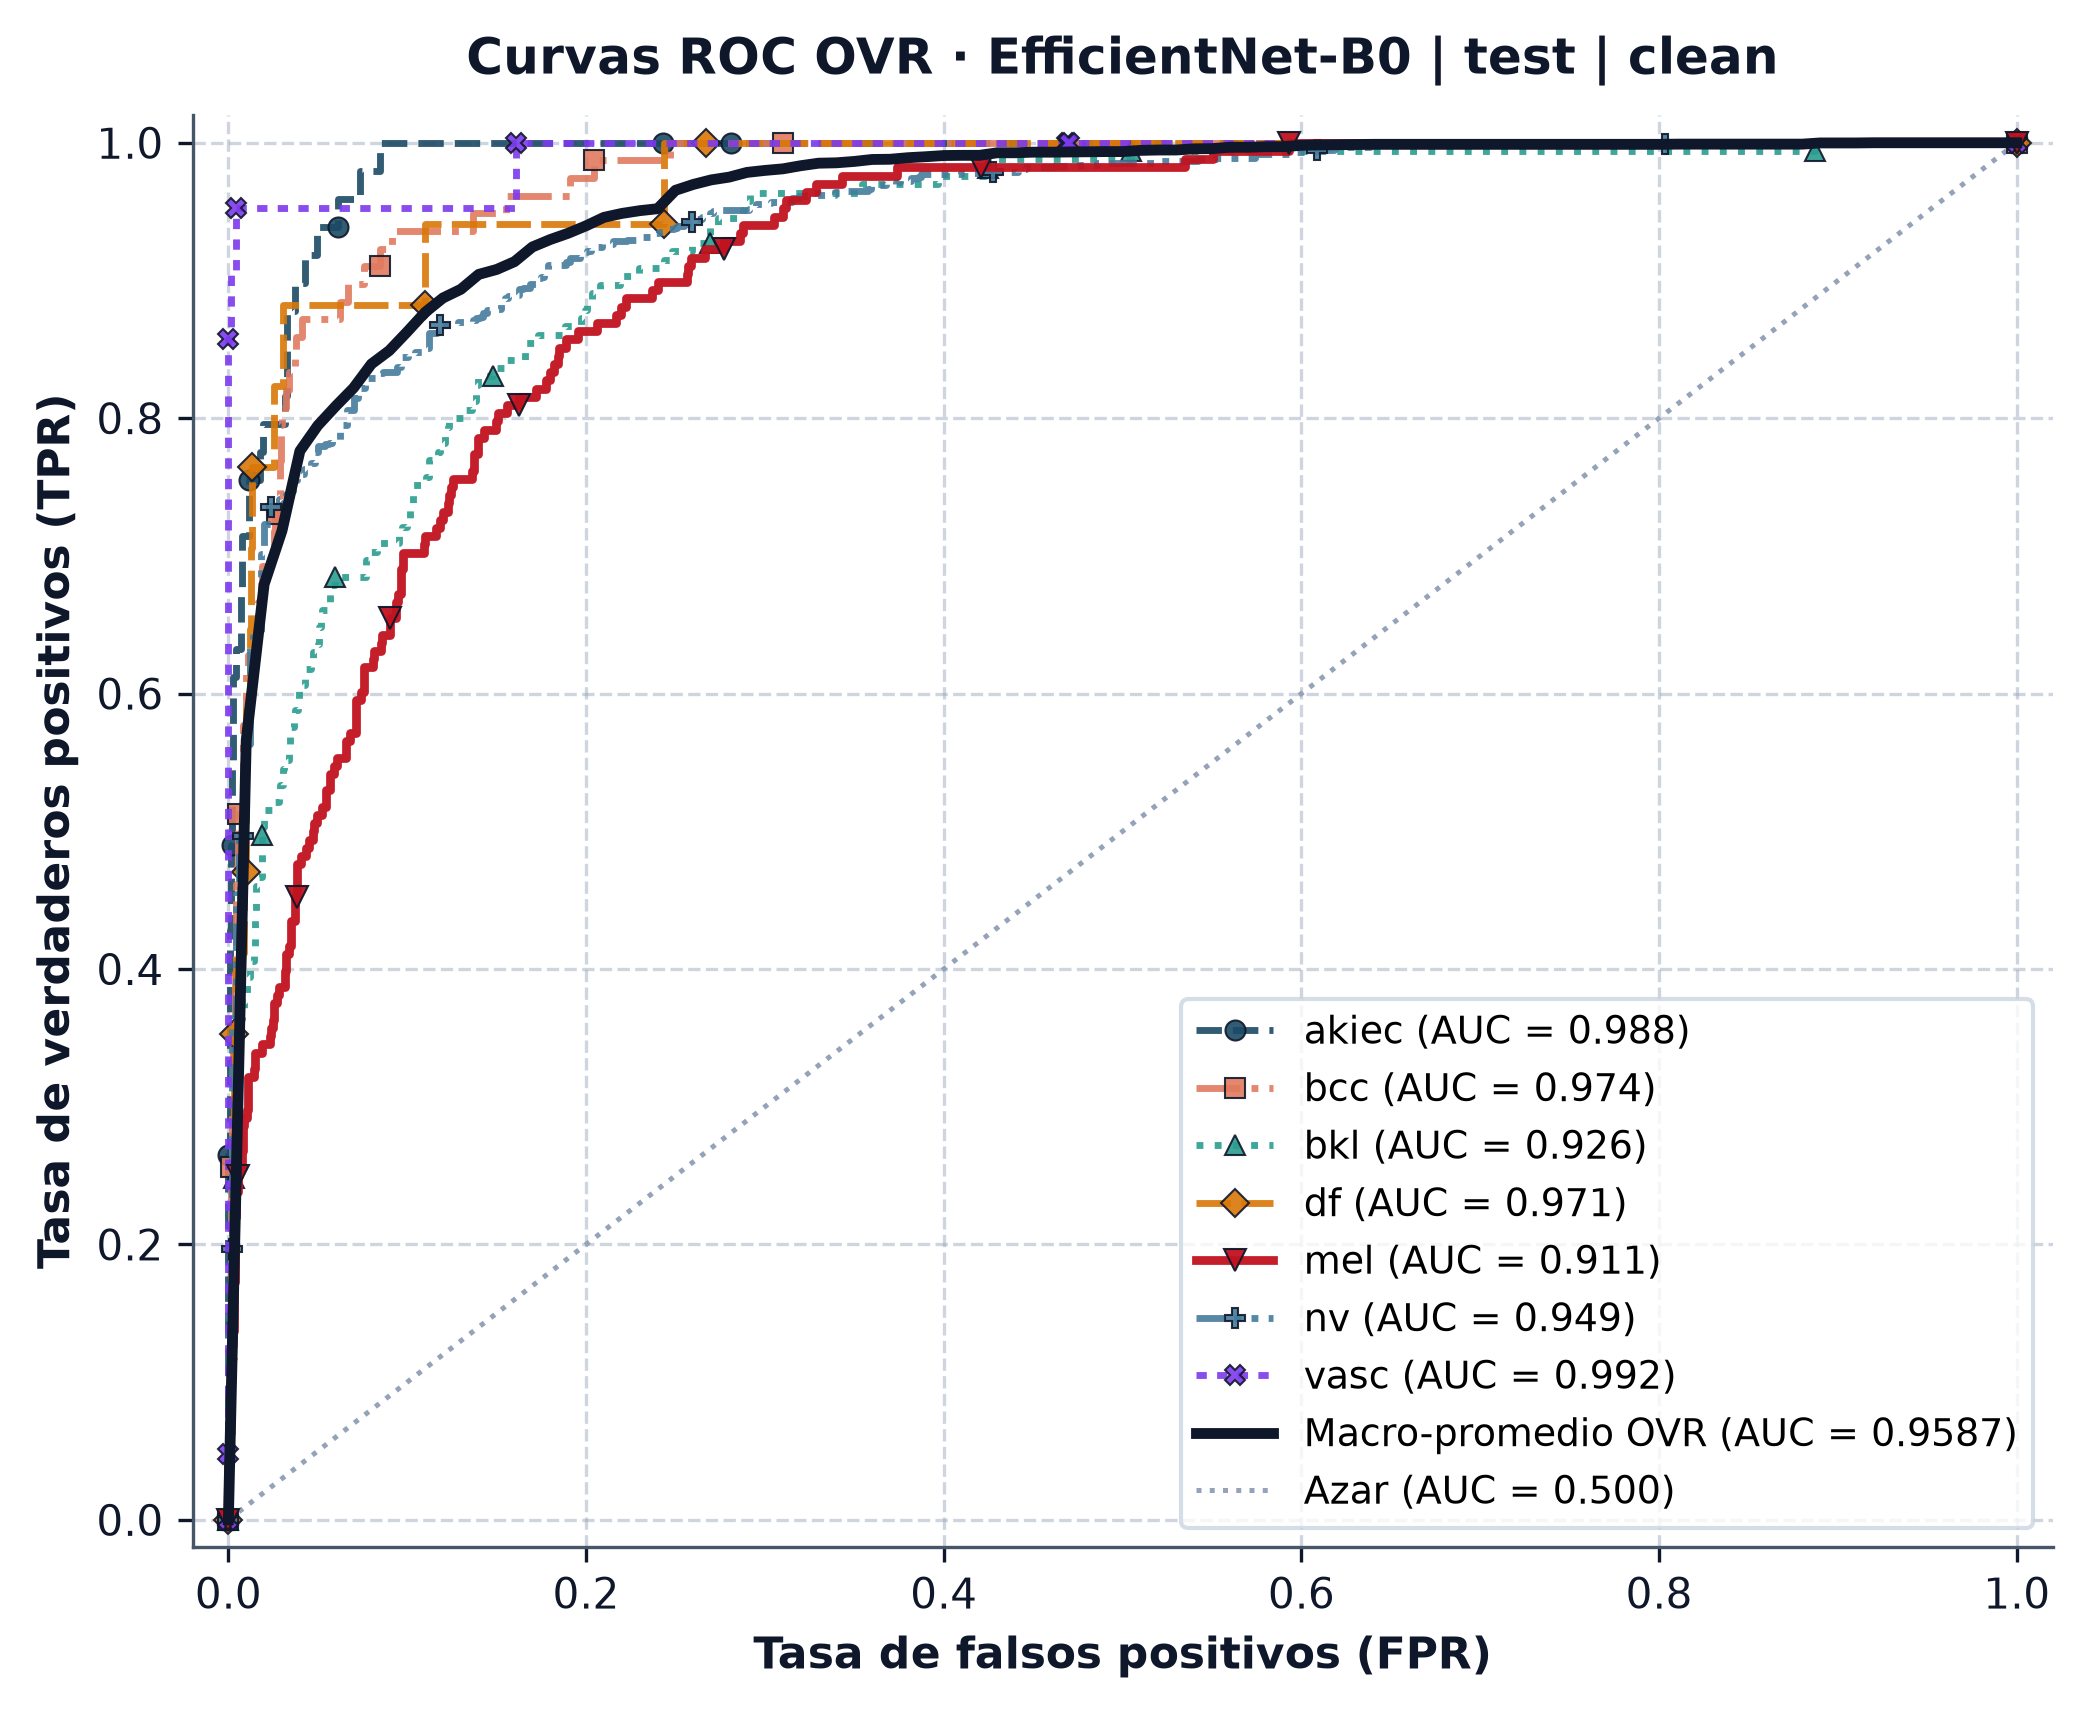
\includegraphics[width=0.78\textwidth]{roc_efficientnet_b0_42_test_clean.png}
\caption{Curvas ROC uno contra el resto (OVR) por clase en \texttt{test} limpio para EfficientNet-B0 (\texttt{seed=42}).}
\label{fig:roc_effnet}
\end{figure}

\begin{figure}[htbp]
\centering
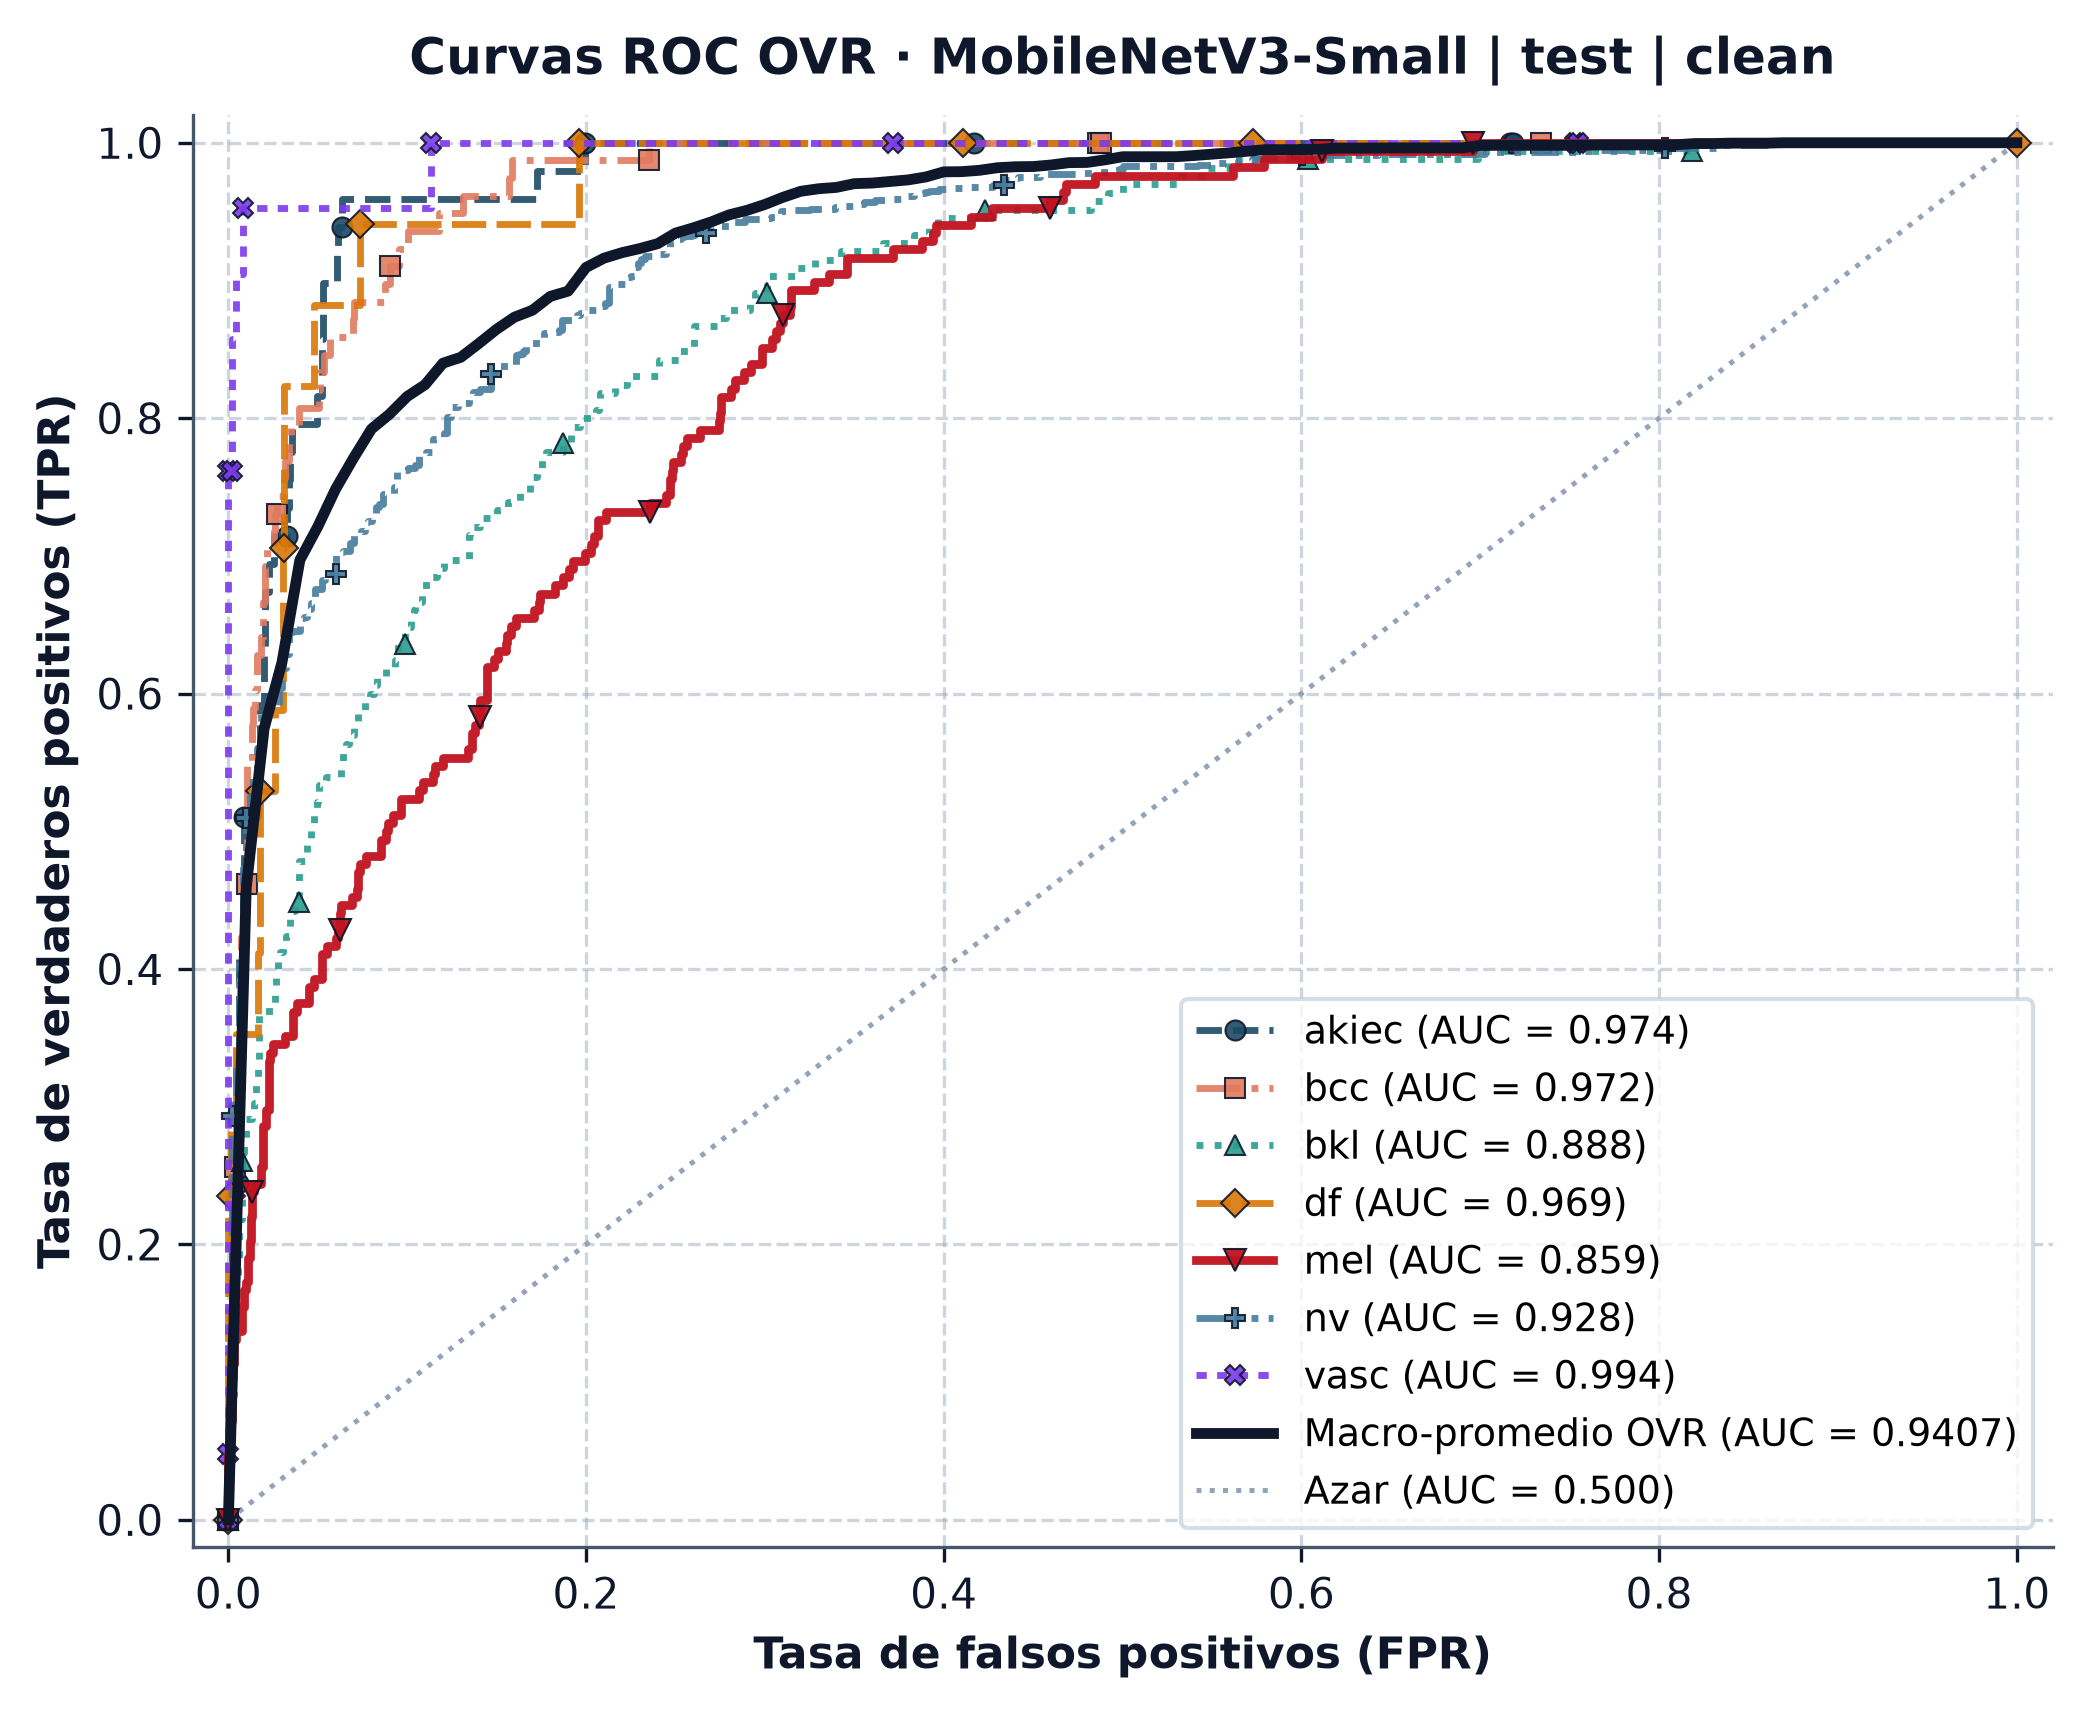
\includegraphics[width=0.78\textwidth]{roc_mobilenet_v3_small_42_test_clean.png}
\caption{Curvas ROC uno contra el resto (OVR) por clase en \texttt{test} limpio para MobileNetV3-Small (\texttt{seed=42}).}
\label{fig:roc_mobilenet}
\end{figure}
\FloatBarrier

Las curvas ROC OVR (Figuras~\ref{fig:roc_comp} y~\ref{fig:roc_resnet}--\ref{fig:roc_mobilenet}) corroboran un alto poder de ordenamiento probabilístico global ($\mathrm{AUC}_{\mathrm{OVR}}$ macro de 0.9596 en ResNet-18, 0.9587 en EfficientNet-B0 y 0.9407 en MobileNetV3-Small). En el análisis individual por clase, \texttt{mel} registra sistemáticamente el AUC más bajo de las siete categorías (0.8947 en ResNet-18, 0.9113 en EfficientNet-B0 y 0.8594 en MobileNetV3-Small), frente a valores superiores a 0.97 en \texttt{vasc}, \texttt{bcc} y \texttt{akiec}, y $\mathrm{AUC}_{\mathrm{OVR}} \ge 0.969$ en \texttt{df} (0.9692 en MobileNetV3-Small, 0.9708 en EfficientNet-B0 y 0.9882 en ResNet-18), lo cual confirma que el solapamiento morfológico de \texttt{mel} con \texttt{nv} y \texttt{bkl} constituye la principal barrera del problema.

\FloatBarrier
\subsection{Comparación de sensibilidad ante ruido, desenfoque y mitigación espacial}
La Tabla~\ref{tab:res_rob} reporta la estabilidad de Macro~F1 y las caídas máximas ($\Delta F1$ y $\Delta\mathrm{Rec.\ mel}$) frente a las cinco condiciones deterministas en \texttt{test}, mientras las Tablas~\ref{tab:res_mit} y~\ref{tab:res_mel_tradeoff} junto con la Figura~\ref{fig:comp_rob} cuantifican tanto la recuperación agregada como el intercambio entre \textit{Precision}, \textit{Recall} y falsos positivos en melanoma sobre \texttt{noise\_005}.

\begin{table}[htbp]\centering\footnotesize
\setlength{\tabcolsep}{2.5pt}
\caption{Comparación de robustez en Macro F1 bajo ruido gaussiano y desenfoque en \texttt{test} ($n=1\,503$).}
\label{tab:res_rob}
\begin{tabularx}{\textwidth}{@{}>{\bfseries}l*{7}{>{\centering\arraybackslash}X}@{}}
\toprule
\textbf{Arquitectura} & \textbf{\texttt{clean}} & \textbf{\texttt{noise\_002}} & \textbf{\texttt{noise\_005}} & \textbf{\texttt{blur\_1}} & \textbf{\texttt{blur\_2}} & \makecell{\textbf{$\Delta F1$}\\\textbf{máx.}} & \makecell{\textbf{$\Delta\mathrm{Rec.}$}\\\textbf{\texttt{mel} máx.}} \\ \midrule
ResNet-18 & \textbf{0.6786} & \textbf{0.4561} & 0.2710 & \textbf{0.5769} & \textbf{0.4895} & +0.4076 & +0.4762 \\
EfficientNet-B0 & 0.6778 & 0.2745 & 0.1201 & 0.5167 & 0.2815 & +0.5577 & +0.6607 \\
MobileNetV3-Small & 0.5700 & 0.3580 & \textbf{0.3079} & 0.5398 & 0.3949 & +0.2621 & +0.3333 \\
\bottomrule
\end{tabularx}
\end{table}

\begin{table}[htbp]\centering\footnotesize
\setlength{\tabcolsep}{2pt}
\caption{Efecto agregado de la mitigación espacial determinista sobre \texttt{noise\_005} en \texttt{test} ($n=1\,503$).}
\label{tab:res_mit}
\begin{tabularx}{\textwidth}{@{}>{\bfseries}l*{9}{>{\centering\arraybackslash}X}@{}}
\toprule
\textbf{Arquitectura} & \multicolumn{3}{c}{\textbf{\texttt{noise\_005} (sin filtro)}} & \multicolumn{3}{c}{\textbf{\texttt{+median\_3}}} & \multicolumn{3}{c}{\textbf{\texttt{+gaussian\_1}}} \\
\cmidrule(lr){2-4}\cmidrule(lr){5-7}\cmidrule(lr){8-10}
 & \textbf{F1} & \makecell{\textbf{Rec.}\\\textbf{\texttt{mel}}} & \textbf{AUC} & \textbf{F1} & \makecell{\textbf{Rec.}\\\textbf{\texttt{mel}}} & \textbf{AUC} & \textbf{F1} & \makecell{\textbf{Rec.}\\\textbf{\texttt{mel}}} & \textbf{AUC} \\ \midrule
ResNet-18 & 0.2710 & 0.1250 & 0.8655 & 0.4624 & 0.6190 & 0.9268 & \textbf{0.5104} & \textbf{0.6905} & \textbf{0.9342} \\
EfficientNet-B0 & 0.1201 & 0.0000 & 0.4839 & 0.4383 & 0.3095 & 0.9090 & 0.4518 & 0.1250 & 0.9187 \\
MobileNetV3-Small & 0.3079 & 0.0833 & 0.8966 & 0.3804 & 0.1964 & 0.9137 & 0.4505 & 0.2381 & 0.9202 \\
\bottomrule
\end{tabularx}
\end{table}

\begin{table}[htbp]\centering\scriptsize
\setlength{\tabcolsep}{3pt}
\caption{Intercambio explícito entre Precision, Recall y falsos positivos en melanoma (\texttt{mel}, $n=168$) bajo \texttt{clean}, \texttt{noise\_005} y mitigación espacial.}
\label{tab:res_mel_tradeoff}
\begin{tabularx}{\textwidth}{@{}>{\bfseries}l>{\ttfamily}l*{5}{>{\centering\arraybackslash}X}c@{}}
\toprule
\textbf{Arquitectura} & \textrm{\textbf{Condición}} & \makecell{\textbf{Macro}\\\textbf{Prec.}} & \makecell{\textbf{Macro}\\\textbf{F1}} & \makecell{\textbf{\texttt{mel}}\\\textbf{Prec.}} & \makecell{\textbf{\texttt{mel}}\\\textbf{Recall}} & \makecell{\textbf{\texttt{mel}}\\\textbf{F1}} & \textbf{TP / FP / FN (\texttt{mel})} \\ \midrule
ResNet-18 & clean & 0.6591 & 0.6786 & 0.5233 & 0.6012 & 0.5596 & 101 / 92 / 67 \\
ResNet-18 & noise\_005 & 0.4003 & 0.2710 & 0.6562 & 0.1250 & 0.2100 & 21 / 11 / 147 \\
ResNet-18 & +median\_3 & 0.6233 & 0.4624 & 0.3675 & 0.6190 & 0.4612 & 104 / 179 / 64 \\
ResNet-18 & +gaussian\_1 & 0.6084 & 0.5104 & 0.3648 & 0.6905 & 0.4774 & 116 / 202 / 52 \\ \midrule
EfficientNet-B0 & clean & 0.6741 & 0.6778 & 0.4868 & 0.6607 & 0.5606 & 111 / 117 / 57 \\
EfficientNet-B0 & noise\_005 & --- & 0.1201 & 0.0000 & 0.0000 & 0.0000 & 0 / 0 / 168 \\
EfficientNet-B0 & +median\_3 & --- & 0.4383 & 0.4906 & 0.3095 & 0.3796 & 52 / 54 / 116 \\
EfficientNet-B0 & +gaussian\_1 & --- & 0.4518 & 0.6364 & 0.1250 & 0.2090 & 21 / 12 / 147 \\ \midrule
MobileNetV3-Small & clean & 0.6474 & 0.5700 & 0.4698 & 0.4167 & 0.4416 & 70 / 79 / 98 \\
MobileNetV3-Small & noise\_005 & --- & 0.3079 & 0.7778 & 0.0833 & 0.1505 & 14 / 4 / 154 \\
MobileNetV3-Small & +median\_3 & --- & 0.3804 & 0.7174 & 0.1964 & 0.3084 & 33 / 13 / 135 \\
MobileNetV3-Small & +gaussian\_1 & --- & 0.4505 & 0.6780 & 0.2381 & 0.3524 & 40 / 19 / 128 \\
\bottomrule
\end{tabularx}
\par\smallskip{\scriptsize\raggedright Nota: los conteos TP/FP/FN de melanoma se calculan directamente sobre el soporte $n_{\mathrm{mel}}=168$ en \texttt{test} a partir de $\mathrm{TP}=n_{\mathrm{mel}}\cdot\mathrm{Recall}$ y $\mathrm{FP}=\mathrm{TP}/\mathrm{Prec.}-\mathrm{TP}$.\par}
\end{table}

\begin{figure}[htbp]
\centering
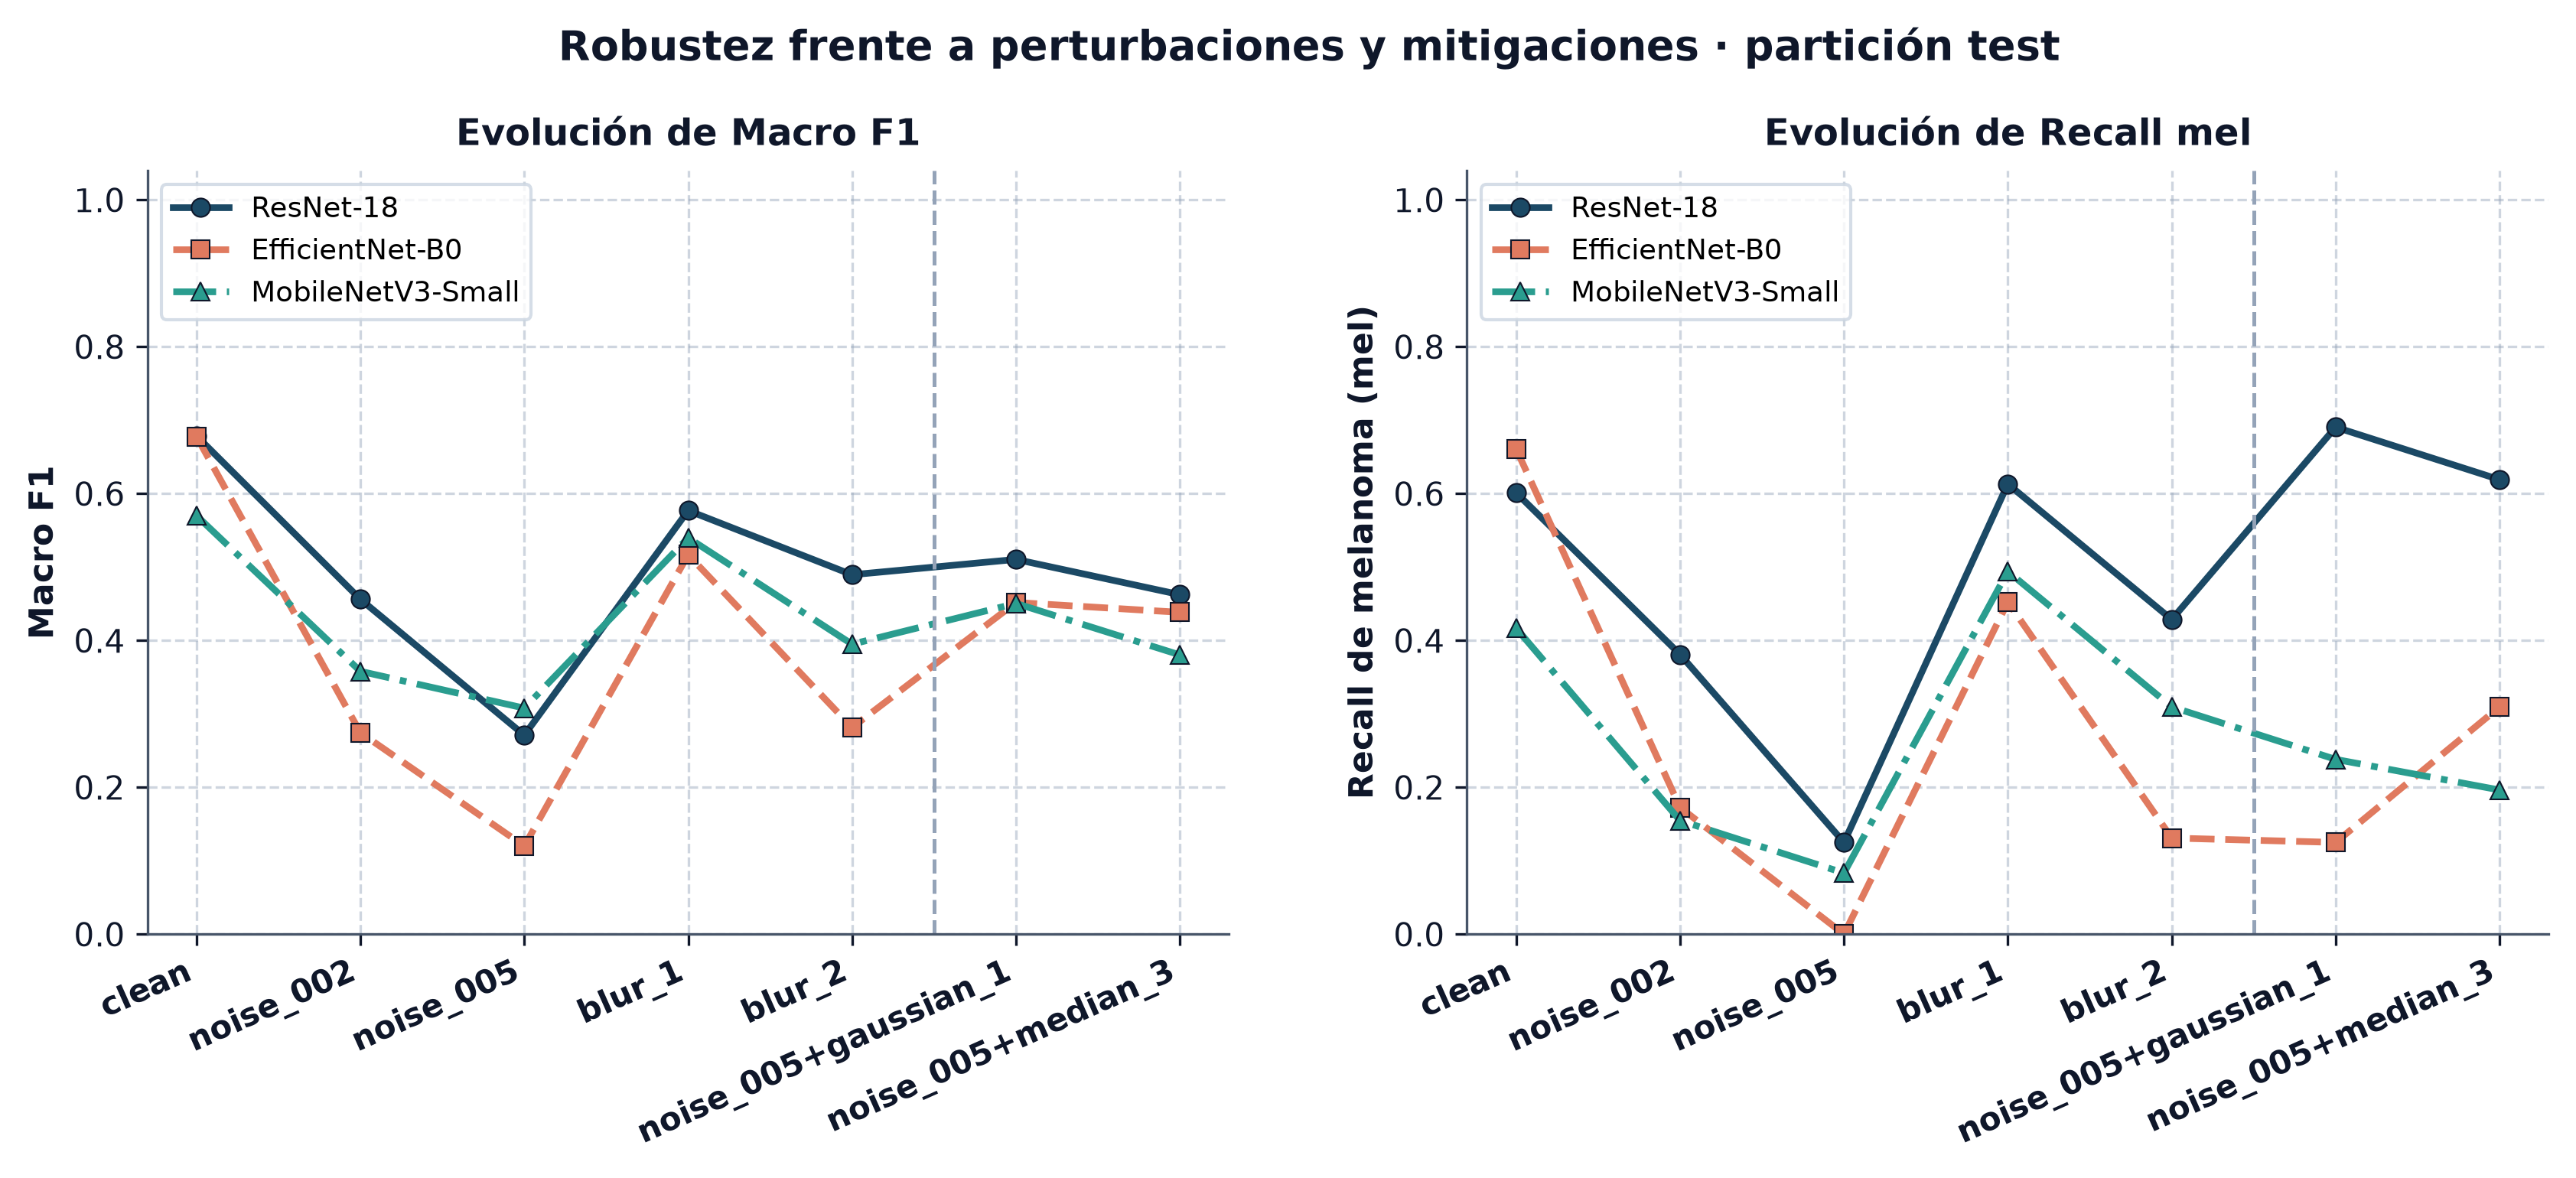
\includegraphics[width=0.96\textwidth]{comparacion_robustez.png}
\caption{Evolución de Macro~F1 (izquierda) y sensibilidad de melanoma (derecha) frente a las cinco condiciones base y las dos variantes de mitigación espacial sobre \texttt{noise\_005}.}
\label{fig:comp_rob}
\end{figure}
\FloatBarrier

La degradación frente a perturbaciones revela contrastes marcados entre arquitecturas:
\begin{itemize}[leftmargin=1.4em,itemsep=3pt]
\item \textbf{Fragilidad severa ante ruido gaussiano:} todas las redes sufren más ante ruido aditivo de alta frecuencia que ante desenfoque moderado. \textbf{EfficientNet-B0} resulta la más vulnerable: cae de 0.6778 a 0.2745 en \texttt{noise\_002} y colapsa hasta 0.1201 en \texttt{noise\_005} ($\Delta F1_{\max}=+0.5577$), anulando por completo la detección de melanoma (\textit{Precision} = 0.0000, \textit{Recall} = 0.0000; $\Delta\mathrm{Rec.\ mel}=+0.6607$; $\mathrm{AUC}_{\mathrm{OVR}}=0.4839$). Como hipótesis interpretativa plausible (pendiente de comprobar mediante ablación), esta caída puede asociarse a una mayor sensibilidad de sus bloques iniciales y módulos de atención de canales SE a texturas de alta frecuencia. MobileNetV3-Small presenta menor caída absoluta ($\Delta F1_{\max}=+0.2621$) y conserva 0.3079 en \texttt{noise\_005}, pero parte de una línea base limpia muy inferior (0.5700), por lo que no constituye una alternativa más capaz.
\item \textbf{Estabilidad relativa ante desenfoque:} \textbf{ResNet-18} mantiene los valores absolutos más altos en \texttt{noise\_002} (0.4561), \texttt{blur\_1} (0.5769) y \texttt{blur\_2} (0.4895), mientras EfficientNet-B0 cae bruscamente ante desenfoque intenso (\texttt{blur\_2}: 0.2815). Como hipótesis interpretativa plausible, las conexiones residuales y filtros iniciales más amplios de ResNet-18 podrían tolerar mejor la atenuación de detalle fino sin perder estabilidad en \textit{logits}.
\item \textbf{Mitigación parcial e intercambio Precision/Recall mediante filtrado espacial (Tablas~\ref{tab:res_mit} y~\ref{tab:res_mel_tradeoff}):} el prefiltrado determinista sin reentrenamiento aporta una ganancia en Macro~F1 sobre \texttt{noise\_005} de \textbf{$+0.14$ a $+0.33$} puntos con \texttt{+gaussian\_1} ($+0.1426$ en MobileNetV3-Small, $+0.2394$ en ResNet-18 y $+0.3317$ en EfficientNet-B0). No obstante, los resultados demuestran que \texttt{+gaussian\_1} constituye una \textbf{mitigación parcial} sujeta a un marcado compromiso operativo: en \textbf{ResNet-18}, \texttt{+gaussian\_1} eleva Macro~F1 de 0.2710 a \textbf{0.5104} (Macro~Prec.\ de 0.4003 a 0.6084), $\mathrm{AUC}_{\mathrm{OVR}}$ de 0.8655 a \textbf{0.9342} y el \textit{Recall} de melanoma de 0.1250 a \textbf{0.6905} (TP sube de 21 a 116), pero a costa de duplicar con creces los falsos positivos respecto a \texttt{clean} (de \textbf{92} a \textbf{202}), reduciendo la \textit{Precision} de melanoma de \textbf{0.5233} a \textbf{0.3648} (F1 \texttt{mel} = 0.4774 vs.\ 0.5596 limpio). De forma análoga, \texttt{+median\_3} eleva el \textit{Recall} de melanoma en ResNet-18 a 0.6190 (TP = 104) con 179 falsos positivos (Precision = 0.3675). En \textbf{EfficientNet-B0}, ambos filtros recuperan el ordenamiento probabilístico global ($\mathrm{AUC}$ sube de 0.4839 a 0.9090 con \texttt{+median\_3} y 0.9187 con \texttt{+gaussian\_1}), pero la cobertura de melanoma sigue deprimida (\textit{Recall} = 0.3095 con \texttt{+median\_3} y 0.1250 con \texttt{+gaussian\_1}). En \textbf{MobileNetV3-Small}, \texttt{+gaussian\_1} alcanza 0.4505 en Macro~F1 y 0.2381 en \textit{Recall} de melanoma (\textit{Precision} = 0.6780). El déficit residual frente a \texttt{clean} obedece al alisado de estructuras dermatoscópicas finas y al desplazamiento de frontera de decisión.
\end{itemize}

\FloatBarrier
\subsection{Síntesis comparativa condicionada al protocolo y hardware}
\begin{tcolorbox}[resBox,title={Recomendación académica condicionada sobre GTX~1650 (\texttt{seed=42}, $n=1\,503$)}]
Bajo la receta compartida (\texttt{configs/base.json}), precisión FP32 y presupuesto de 4~GiB de VRAM en GTX~1650, \textbf{ResNet-18} ofrece el mejor compromiso observado desempeño--latencia en HAM10000: registra Macro~F1 = \textbf{0.6786} (Macro~Prec.\ = 0.6591), \textit{Balanced Accuracy} = \textbf{0.7174}, \textit{Accuracy} = \textbf{0.8031} y $\mathrm{AUC}_{\mathrm{OVR}}$ = \textbf{0.9596}, entrena en menor tiempo (\textbf{127.5~s/época}), infiere con mediana \texttt{forward()} de \textbf{7.22~ms} (P95 = 8.09~ms; rango entre corridas $6.86$--$9.46$~ms) con 434.2~MiB de VRAM, conserva mejores métricas bajo desenfoque y ruido moderado, y alcanza la mayor recuperación tras mitigación parcial (\textbf{0.5104} Macro~F1 con \texttt{+gaussian\_1}, con el compromiso de elevar falsos positivos en melanoma de 92 a 202).\\[4pt]
Sin embargo, la diferencia de 0.00084 en Macro~F1 frente a \textbf{EfficientNet-B0} (0.6778; Macro~Prec.\ = \textbf{0.6741}) \textbf{no demuestra superioridad estadística ni equivalencia} (IC95\% \textit{bootstrap} pareado por $1\,118$ \texttt{group\_id}: $[-0.0429, +0.0464]$). EfficientNet-B0 obtiene la mayor sensibilidad limpia en melanoma (\textbf{0.6607}) y F1 en \texttt{akiec} (0.7143), pero requiere mayor latencia (24.60~ms; rango $22.49$--$34.82$~ms), mayor VRAM (805.7~MiB) y exhibe extrema fragilidad frente a ruido aditivo. \textbf{MobileNetV3-Small} minimiza memoria (211.8~MiB), pero penaliza las categorías minoritarias (Macro~F1 = 0.5700; \texttt{mel} recall = 0.4167; \texttt{akiec} F1 = 0.2667) sin ofrecer ventaja de velocidad en esta GPU (22.40~ms; rango $15.26$--$22.40$~ms). Esta recomendación queda condicionada al protocolo, semilla única y hardware evaluado, y \textbf{no constituye validez ni indicación clínica}.
\end{tcolorbox}
\FloatBarrier
